\chapter{El problema inverso}%
\lhead{\thepage}
\rhead{\textit{El problema inverso}} \\
\vspace{0.01\textheight}
\label{sec:inverso}
%\pagebreak

En las secciones previas abordamos el problema directo de transporte 
de radiación en la materia mediante la ETR. En síntesis, el problema 
directo consta de, dados los parámetros ópticos $a(\x)$, $b(\x)$, la función  
de fase $\eta(\hth\cdot \hth')$, la velocidad de la luz en el medio participante 
$c$, las fuentes internas $s$ y las condiciones iniciales y de contorno, 
encontrar la solución $\ut$ a la ecuación~\eqref{eq:RTE}.

Para el problema inverso en tomografía óptica, alguno de los parámetros 
ópticos es desconocido, 
o conocido sólo parcialmente, y se dispone de mediciones experimentales 
de detectores colocados en el contorno del dominio que se quiere analizar. 
A partir de las mediciones experimentales de estos detectores, 
el objetivo es la reconstrucción de uno o más de los parámetros ópticos. 
En el caso de tomografía por fluorescencia y tomografía de bioluminiscencia, lo que se intenta reconstruir 
son las fuentes $s$ en la ec.~\eqref{eq:RTE}~\cite{Klose2005,Klose2009,Ren2010}, 
que vienen relacionadas a los coeficientes de absorción de los 
cromóforos y fluoróforos. 

En el contexto de esta tesis, nos limitaremos a la reconstrucción del 
coeficiente de absorción, $a(\x)$. La reconstrucción de dicho coeficiente 
encuentra aplicaciones en tomografía de fluorescencia, y en tomografía óptica. 
La reconstrucción de las propiedades de absorción en tomografía óptica 
 permite la identificación de tumores~\cite{Zhu2005,Zhu2010,Fujii2016b}, 
la obtención de imágenes funcionales del cerebro humano~\cite{Boas2001,bluestone2001,Arridge1999}, 
y la caracterización de diferentes constituyentes del tejido 
humano para la obtención de imágenes en medicina. En 
este trabajo nos enfocamos en la reconstrucción del coeficiente 
de absorción, pero los algoritmos y las estrategias propuestas 
pueden ser fácilmente generalizadas para la reconstrucción 
de otros parámetros. 

Generalmente, para aplicaciones 
en diagnostico y monitoreo en el tratamiento de tumores, 
se asume cierta información previa 
para el coeficiente de dispersión, 
$b(\x)$, obtenida por técnicas de obtención 
de imágenes de alta resolución~\cite{Althobaiti2017,Guven2003} \eg Resonancia Magnética. 
Este conocimiento previo obtenido por otras técnicas, también brinda 
información limitada en el parámetro óptico de absorción $a(\x)$, 
como pueden ser los coeficientes de absorción para ciertos tejidos óseos, 
o el aire en regiones como la traquea del cuello humano, como también 
se conocen cotas superiores e inferiores para dicho parámetro, 
lo que permite restringir el espacio de funciones donde se busca minimizar 
la función objetivo. El uso de técnicas de alta resolución, como la Resonancia 
Magnética, posee ciertas limitaciones, como el alto costo, la baja disponibilidad 
de este tipo de aparatos 
(lo que impone una dificultad a la hora de seguir la evolución de un tratamiento 
asistido por diagnóstico de imágenes), y adicionalmente los dispositivos 
utilizados en tomografía óptica son portables, lo que permite tenerlos disponibles 
para su uso en diversas situaciones. En la figura~\ref{fig:esquemainv} esquematizamos los problemas directos e inverso, tal como son 
tratados en esta tesis. 


\begin{figure}[h!]
\centering
  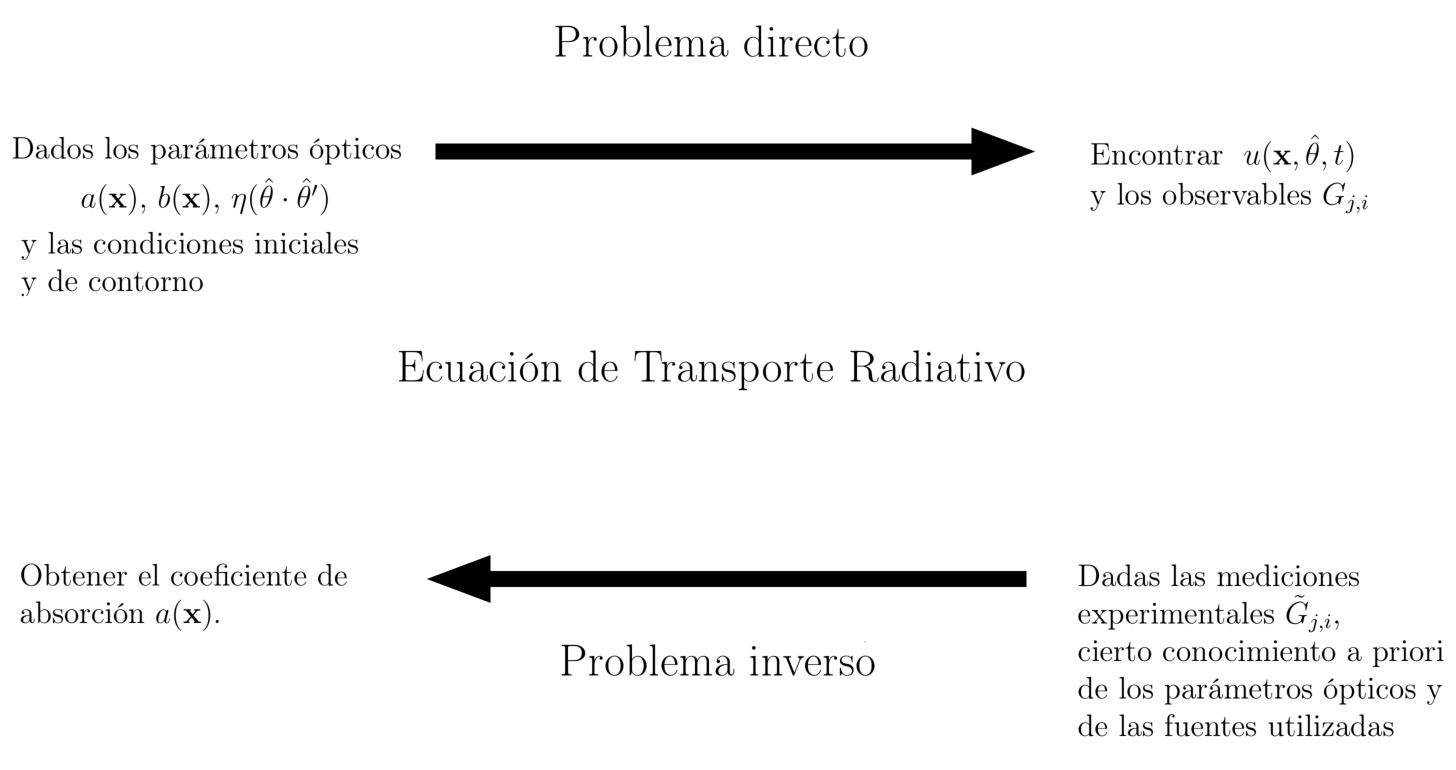
\includegraphics[width=\linewidth]{figuras/inv.pdf}\\
  \caption{
Grafico esquemático de los problemas directo e inverso, tal como son considerados 
en esta tesis.}
 \label{fig:esquemainv}
\end{figure}
Para la resolución del problema inverso, utilizamos el esquema \textit{MOBIR}, 
presentado en la sección siguiente. 

\section{El esquma \textit{MOBIR}}

\begin{wrapfigure}{l}{0.48\textwidth}
  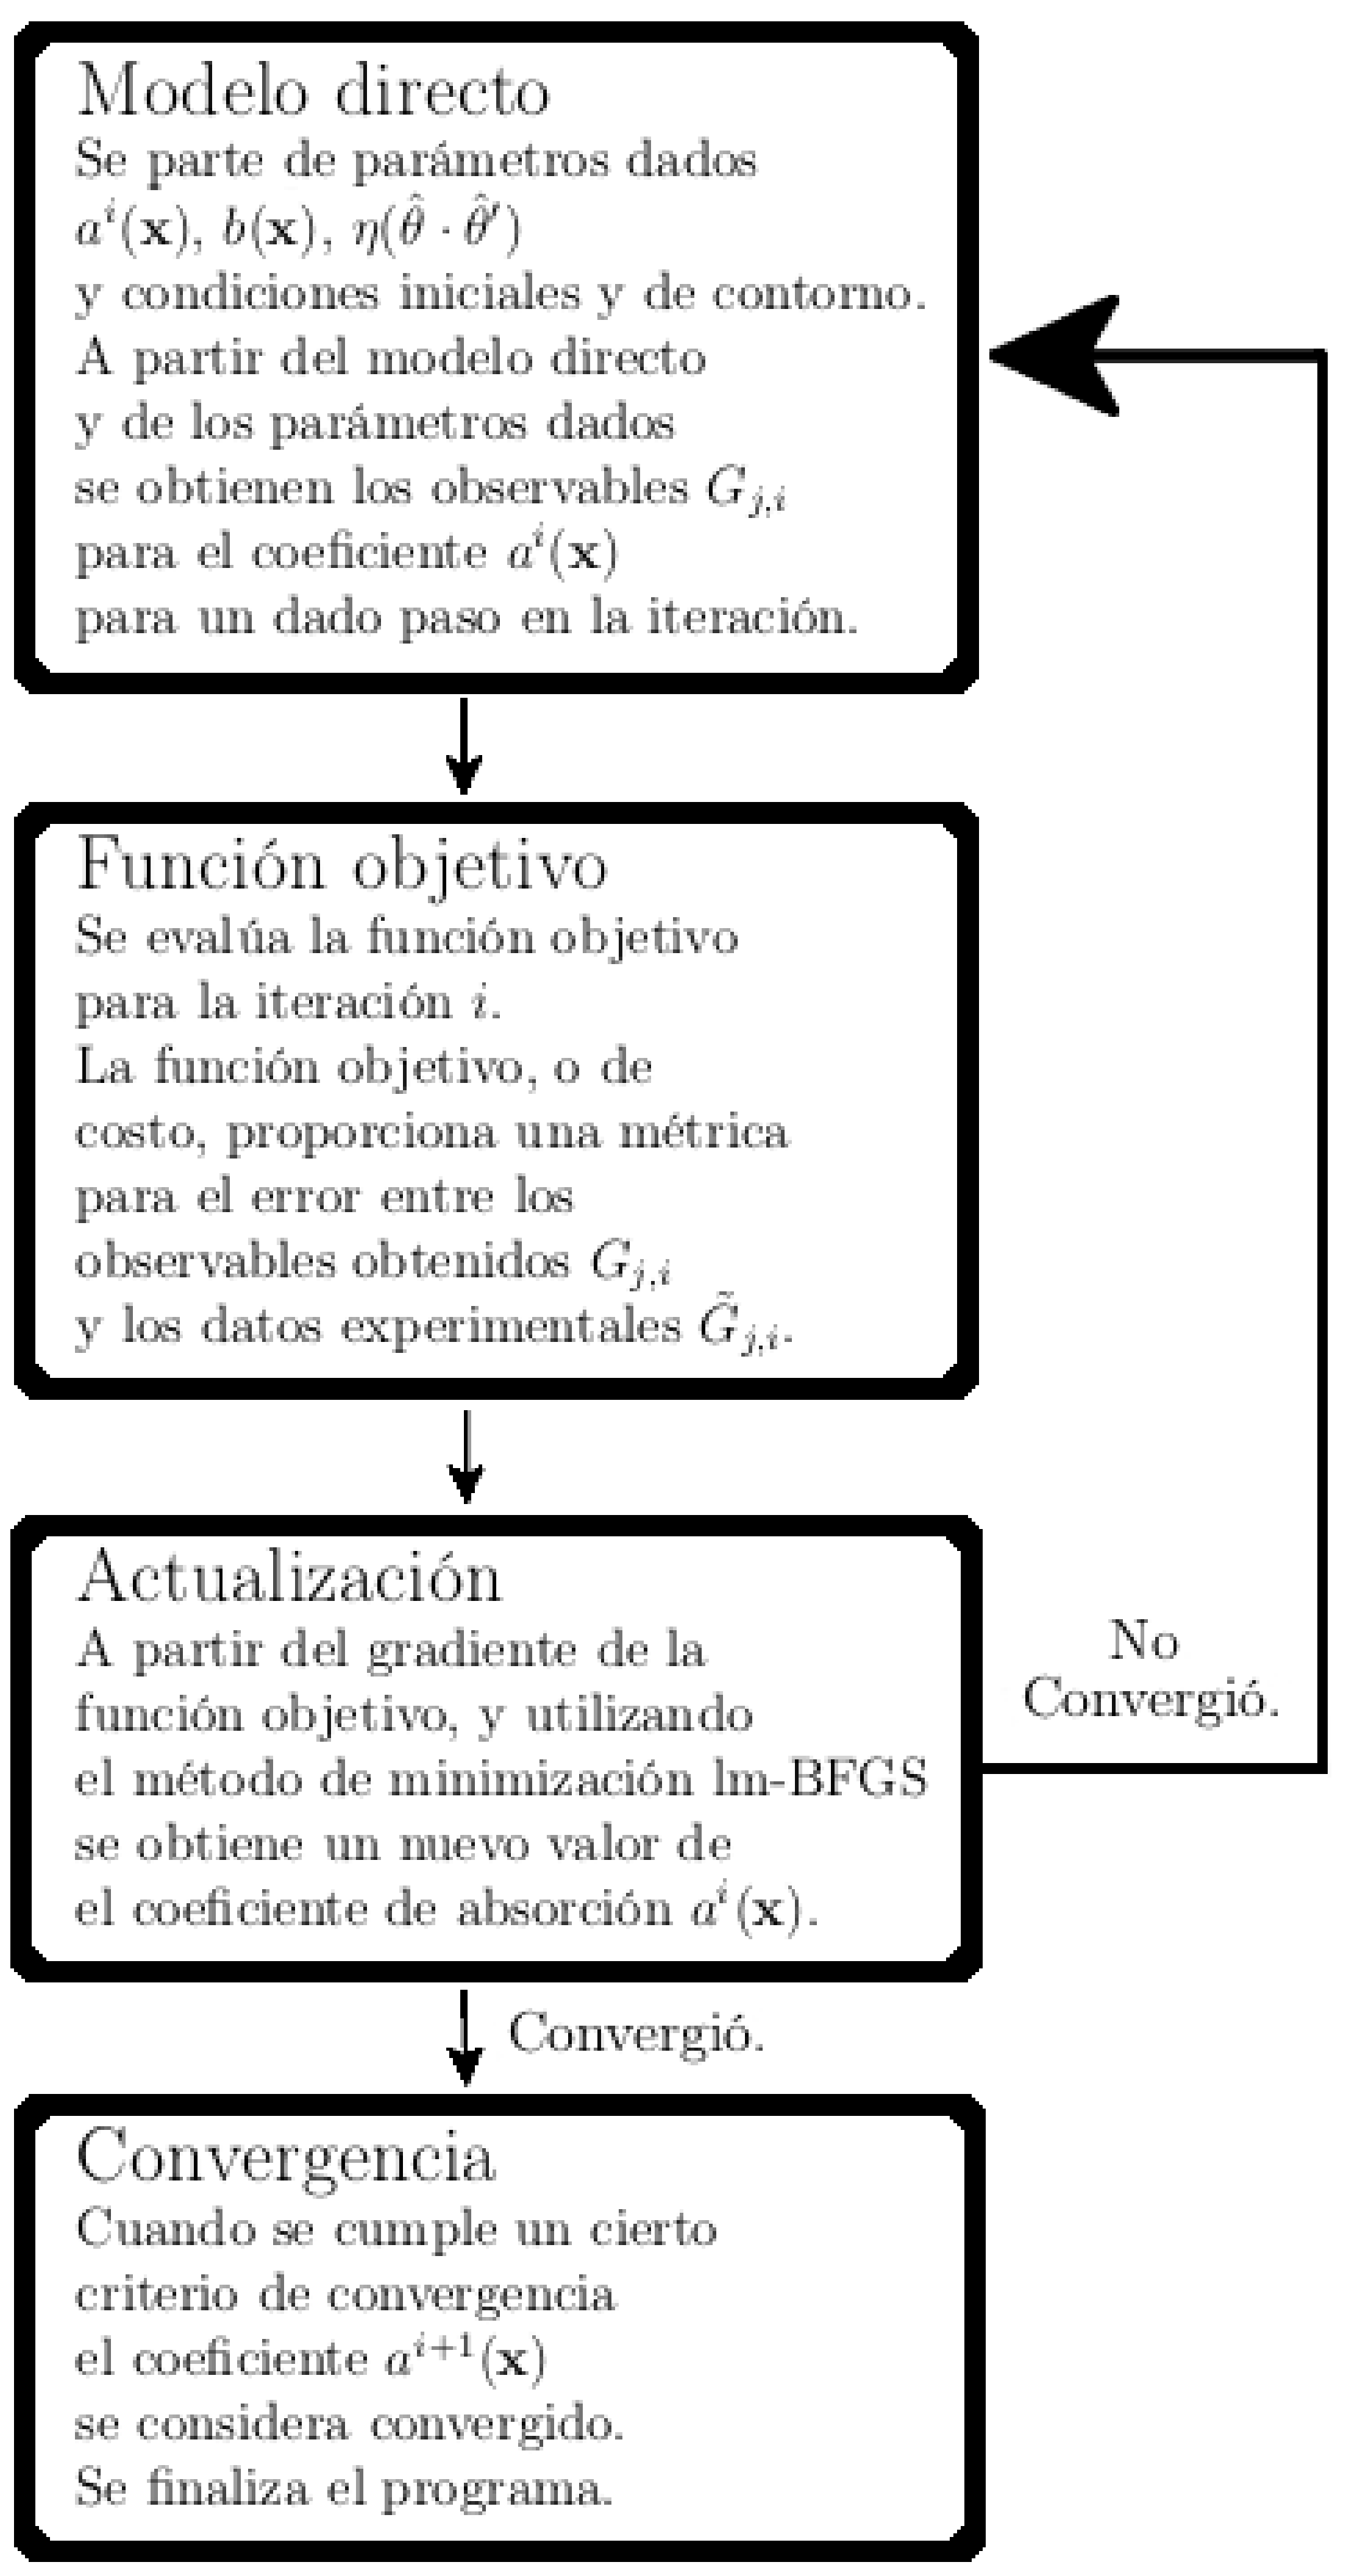
\includegraphics[width=0.48\textwidth]{figuras/mobir.eps}\\
  \caption{Esquema  MOBIR. El modelo directo es utilizado para obtener los observables simulados. Se evalúa el error entre los datos experimentales y los simulados por medio de la función objetivo. 
  Luego, utilizando un método de minimización, se actualiza el coeficiente $a(\x)^{i+1}$ a 
  ser utilizado en la iteración subsiguiente, hasta cumplir 
  un cierto criterio de convergencia. }
 \label{fig:mobir}
\end{wrapfigure}

En este tesis desarrollamos un algoritmo tipo MOBIR~\cite{Hielscher1999,Kim2010} (del inglés, {\em Model Based Iterative Image  
Reconstruction}). Este tipo de esquemas se basan en un modelo físico, y un método de minimización 
iterativo para la reconstrucción del parámetro deseado en el problema inverso.

El modelo físico utilizado es la Ecuación de Transporte Radiativo~\eqref{eq:RTE}. 
Para la minimización del funcional objetivo (que será introducido en una sección posterior) emplearemos el método de minimización 
de Broyden–Fletcher–Goldfarb–Shanno (BFGS) con uso de memoria reducido 
(lm-BFGS, de su sigla en inglés)~\cite{Byrd1995}. 

El problema inverso en tomografía óptica es resuelto como un problema de optimización 
no lineal. A partir de un valor inicial para el coeficiente de absorción $a(\x)^0$, 
el coeficiente de absorción es buscado de forma iterativa, actualizando su valor 
en cada iteración mediante el método lm-BFGS, el cual es un caso particular 
de los métodos de cuasi-Newton~\cite{Nocedal2006,Klose2003QN,Ren2006}. 
Partiendo del valor inicial $a^0(\x)$, el cual en general es estimado 
a partir de información obtenida de manera previa por otros métodos de imagenes, 
el coeficiente de absorción es 
\clearpage
\noindent actualizado en cada paso de la iteración $i+1$, según~\cite{Klose2003QN}
\begin{equation}
\mathbf{a}^{i+1}(\x)=\mathbf{a}^{i}(\x)+\alpha^i  \mathbf{d}^i(\x)
\label{eq:update}
\end{equation}
donde $\mathbf{a}^{i}(\x)$ debe ser interpretado como el 
vector obtenido a partir de el coeficiente de absorción en el 
dominio espacial $\Omega$  
discretizado, con $\alpha^i$ el largo del paso de Newton (que lo consideraremos 
en general $\alpha^i=1$), y $\mathbf{d}^i(\x)$ 
la dirección de descenso. En el caso del método de Newton (o {\em steepest descent}), la dirección de 
descenso vendrá dada por el gradiente $\mathbf{d}^i=-\nabla_a $ de la función objetivo $g$ (que será definida posteriormente). 
En el contexto de esta tesis emplearemos el método lm-BFGS, ya que este método a 
mostrado ser eficiente en el contexto de tomografía óptica~\cite{Klose2003QN,Ren2006,
Prieto2017}. 

\section{El método de minimización BFGS}
\label{sec:BFGS}
Siguiendo a Nocedal~\cite{Nocedal2006}, el método BFGS parte de considerar la expansión de Taylor a segundo orden de la función objetivo 
que buscamos minimizar, la cual estará evaluada para el coeficiente $\mathbf{a}(\x)$,  
lo notaremos, por simplicidad  $g[\mathbf{a}]$

\begin{equation}
g[\mathbf{a}^i+ \mathbf{d}^i]\approx g[\mathbf{a}^i]+ (\mathbf{d}^i)^T \nabla_a g[\mathbf{a}^i]+\frac{1}{2}(\mathbf{d}^i)^T \nabla_a^2 g[\mathbf{a}^i+t\mathbf{d}^i] \mathbf{d}^i=m(\mathbf{d}^i).
\label{eq:Taylor}
\end{equation}
donde $t \in (0,1)$, y $(\mathbf{d}^i)^T$ indica el vector traspuesto a $\mathbf{d}^i$.
Además, si $g$ es al menos dos veces diferenciable se cumple qué 
\begin{equation}
\nabla_a g[\mathbf{a}^i+ \mathbf{d}^i]\approx \nabla_a g[\mathbf{a}^i]+\int_0^1\nabla_a^2 g[\mathbf{a}^i+t\mathbf{d}^i] \mathbf{d}^idt 
\label{eq:Taylor2}
\end{equation}
para algún $t \in (0,1)$.
Exigiendo que se anule la derivada de $m(\mathbf{d^i})$, se llega la dirección de Newton, dada por
\begin{equation}
\mathbf{d}^i=-(\nabla_a^2 g^i )^{-1} \nabla_a g^i.
\label{eq:direccion}
\end{equation}
El principal obstaculo para la aplicación de la dirección de Newton es la 
necesidad de calcular la inversa del Hessiano de la función objetivo, $\nabla_a^2 g^i$, 
lo cual en tomografía óptica, debido a la alta dimensionalidad de la ETR, puede 
resultar extremadamente costoso. 

Por este motivo, el método BFGS implementa una aproximación del Hessiano de la función objetivo (mas concretamente, 
a la inversa del Hessiano) que 
es actualizada a cada paso de la iteración. Sumando y restando el término $ \nabla_a^2 g \mathbf{d}^i$ en la ecuación~\eqref{eq:Taylor2} se llega a
\begin{equation}
\nabla_a g[\mathbf{a}^i+ \mathbf{d}^i]\approx \nabla_a g[\mathbf{a}^i]+ \nabla_a^2 g[\mathbf{a}^i]\mathbf{d}^i + \int_0^1   \left( \nabla_a^2 g[\mathbf{a}^i+t\mathbf{d}^i]-\nabla_a^2 g[\mathbf{a}^i] \right)\mathbf{d}^idt
\label{eq:Taylor3}
\end{equation}
Dado que se asume la continuidad de $\nabla_a g$, el término de la integral 
es $o(||\mathbf{a}^{i+1}-\mathbf{a}^{i}||)$. Tomando $\mathbf{d}^i=\mathbf{a}^{i+1}-\mathbf{a}^{i}$ se llega a la relación
\begin{equation}
\begin{split}
\begin{aligned}
\nabla_a g[\mathbf{a}^{i+1}] &\approx \nabla_a g[\mathbf{a}^i]+ \nabla_a^2 g[\mathbf{a}^{i+1}-\mathbf{a}^i]  + o(||\mathbf{a}^{i+1}-\mathbf{a}^{i}||).\\
\therefore \nabla_a^2 g[\mathbf{a}^{i+1}-\mathbf{a}^i]& \approx \nabla_a g[\mathbf{a}^{i+1}]  - \nabla_a g[\mathbf{a}^{i}].
\end{aligned}
\end{split}
\label{eq:Taylor4}
\end{equation}
Esta última relación nos permite aproximar el Hessiano utilizando las derivadas de 
la función objetivo obtenidos para dos iteraciones sucevias. 
La inversa del Hessiano de la función objetivo es aproximada exigiendo que se cumpla la última relación en~\eqref{eq:Taylor4}, que puede escribirse 
\begin{equation}
(B^{i+1})^{-1}y^i=s^i,
\label{eq:Taylor5}
\end{equation}
con $s_i=  \mathbf{a}^{i+1}-\mathbf{a}^{i}$ y $y^i=\nabla_a g[\mathbf{a}^{i+1}]  - \nabla_a g[\mathbf{a}^{i}]$. La fórmula BFGS para actualizar el Hessiano en cada iteración viene dada por~\cite{Nocedal2006}
\begin{equation}
(B^{i+1})^{-1}=(V^i)^T (B^{i})^{-1}V^i + \rho^i s^i (s^i)^T  ,
%B^{i}-\frac{B^{i}s^i (s^i)^T B^i }{(s^i)^TB^i s^i}+ \frac{y^i (y^i)^T}{(y^i)^T s^i}
\label{eq:HBFGS}
\end{equation}
la cual cumple la relación~\eqref{eq:Taylor5}, donde $\rho^i=\frac{1}{(y^i)^T s^i}$ 
y $V^i=\id - \rho^i y^i (s^i)^T$. 
La dirección de descenso, finalmente, se obtiene de la ecuación~\eqref{eq:direccion} reemplazando 
el Hessiano por su aproximación $B^i$
\begin{equation}
\mathbf{d}^{i}=-(B^{i})^{-1} \nabla_a g[\mathbf{a}^i]. 
\label{eq:HBFGS2}
\end{equation}

\subsection{El método de uso de memoria limitada lm-BFGS}
\label{sec:lmBFGS}
En nuestro algoritmo para la resolución del problema inverso, el coeficiente 
de absorción es actualizado en cada iteración utilizando la relación 

\begin{equation}
\mathbf{a}^{i+1}(\x)=\mathbf{a}^{i}(\x)-(B^{i})^{-1} \nabla_a g[\mathbf{a}^i]
\label{eq:update2}
\end{equation}
Debido a que la aproximación a la inversa del Hessiano, $(B^i)^{-1}$, en tomografía óptica es una matriz 
que para el problema 2D discretizado, con $N_x \times N_y$ puntos 
por cada coordenada espacial tendrá dimensiones  $B^i\in \mathbb{R}^{N_x \times N_y}$, 
la manipulación y almacenamiento de esta matriz puede ser sumamente costosa. Por ello, 
para evitar la manipulación y el almacenamiento de esta matriz, se utiliza 
una versión aproximada de $(B^i)^{-1}$, para la cual se almacenan los vectores $\{s^k, y^k\}$, 
$k=i-m,...,i-1$ para un dado número de puntos $m$ previos a la iteración $i$-esima. 
Para esto se utiliza una aproximación inicial al Hessiano $(B^i)^{-1}_0$
\begin{equation}
(B^i)^{-1}_0=\gamma^i \id,\quad \quad \gamma^i=\frac{(s^{i-1})^T y^{i-1}}{(y^{i-1})^Ty^{i-1}},
\label{eq:initHess}
\end{equation}
y utilizando la ecuación~\eqref{eq:HBFGS} se tiene la relación de recurrencia
\begin{equation}
\begin{split}
\begin{aligned}
(B^{i+1})^{-1}=&(V^{i-1})^T...V^{i-m})^T) (B^i)^{-1}_0 (V^{i-m}...V^{i-1})  \\
&+\rho^{i-m} (V^{i-1})^T...V^{i-m+1})^T)s^{i-m} (s^{i-m})^T(V^{i-m+1}...V^{i-1+1}) \\
&+\rho^{i-m+1} (V^{i-1})^T...V^{i-m+2})^T)s^{i-m+1} (s^{i-m+1})^T(V^{i-m+2}...V^{i-1}) \\
&+...\\
&+\rho^{i-1} s^{i-1} (s^{i-1})^T. 
\end{aligned}
\end{split}
\label{eq:HBFGSrec}
\end{equation}
de donde se tiene el algoritmo~\eqref{algbfgs}~\cite{Byrd1995,Nocedal2006}

\begin{algorithm}
\caption{lm-BFGS}\label{algbfgs}
\begin{algorithmic}[1]
\State dados $m$, $\mathbf{a}^i$, y $\nabla_a g[\mathbf{a}^i]$
\State  $q = \nabla_a g[\mathbf{a}^i]$
\State \textbf{para} $k=i-1,i-2,\ldots,i-m$ hacer 
\State \hskip 0.75em $\alpha^k  = \rho^k (s^k)^T q$,
\State \hskip 0.75em $q  = q- \alpha^k y^k$,
\State \textbf{terminar}
\State $r = (B_0^k)^{-1} q$,
\State \textbf{para} $k=i-m,i-m+1,\ldots,i-1$ hacer 
\State \hskip 0.75em $\beta  = \rho^k (y^k)^T r$,
\State \hskip 0.75em $r  = r+s^k(\alpha^k-\beta)$,
\State \textbf{terminar}
\State Finalizar programa, con $(B^k)^{-1}\nabla_a g[\mathbf{a}^k]=r$.
\end{algorithmic}
\end{algorithm}  
  
En esta tesis utilizaremos el algoritmo lm-BFGS para encontrar 
el mínimo de la función objetivo. En todos los casos, usaremos el valor 
de $m=5$, y se parte de un coeficiente inicial $a^0(\x)$ dado 
por cierto conocimiento obtenido previamente, como puede ser la imagen 
de resonancia magnética de un cuello humano utilizada en la sec.~\ref{sec:inverseres}.
Adicionalmente, es posible incluir cotas para el coeficiente 
de absorción que deseamos reconstruir, de forma tal que 
el proceso de minimización sea realizado 
en un subespacio tal que $a^l(\x)\leq a^i(\x) \leq a^u(\x)$, de forma 
tal que el coeficiente de absorción, para cada punto espacial $\x$ se encuentre 
restringido por las cotas inferior $a^l(\x)$ y superior $a^u(\x)$. Esto restringe el espacio de soluciones posibles, permitiendo explotar información a priori obtenida por otros métodos de imágenes. 
Una condición física que debe cumplirse siempre es que la cota inferior 
para el coeficiente de absorción cumpla $a^l(\x)\geq 0$. Similarmente, 
se conocen cotas superiores para el coeficiente de absorción, y además, 
puede utilizarse los valores conocidos de $a(\x)$ como cotas sobre 
aquellos tejidos donde se sabe que la inclusión no puede ocurrir, 
o si, por la naturaleza del diagnóstico que se está realizando, 
se espera que una dada inclusión 
se encuentre dentro de cierto tipo de tejido, restringiendo mediante cotas 
la reconstrucción para que ocurra dentro del tejido esperado, fijando los 
valores para el resto de los tejidos, como puede ser, la existencia de 
una región de absorción y dispersión nula en la traquea para el cuello 
humano, o las regiones óseas para el caso en el que se intenta dar un diagnóstico 
para un tipo de tumor específico, como lo puede ser para el cáncer de tiroides, 
donde se sabe que el tumor se encontrará localizado en el tejido blando. 
El procedimiento por el cual se imponen dichas cotas en los coeficientes 
puede encontrarse en la ref.~\cite{Byrd1995}. 

\section{El operador de transporte y otras definiciones preliminares}
En esta sección, haremos uso del operador de transporte, el cual definimos
según
\begin{equation}
\begin{split}
\mathcal{T}[u]=\frac{1}
{c}\frac{\partial \ut}{\partial t} + \hth \cdot \nabla \ut&+a(\x)\ut\\
&+b(\x)\left[\ut - \int_{S^1}\eta(\hth\cdot\hth ') u(\x,\hth',t) d\theta'\right],
\end{split}
\label{eq:Toper}
\end{equation}
donde se hizo explícita la dependencia del operador de transporte $\mathcal{T}$ 
con respecto a $\ut$. 

Consideramos el problema ETR de valores iniciales y condiciones 
de contorno
\begin{equation}
\begin{split}
\begin{aligned}
&\mathcal{T}\big[u\big]=0, \;  (\x,\hth)  \in \Omega\times S^1\\
&u(\x,\hth,t=0)=0, \;  (\x,\hth)  \in \Omega\times S^1 \\
&u(\x,\hth,t)=f(\hth \cdot \hnu) u(\x,\hth_r,t) + q(\x,\hth,t) , \; (\x,\hth) \in \Gamma_-
\end{aligned}
\end{split}
\label{eq:RTEt}
\end{equation}
donde todas las cantidades fueron definidas en la sección~\ref{sec:ETR}.


Para concluir esta sección, mencionamos la ``función ventana''~\cite{Bruno2014}
\begin{equation}
\begin{aligned}
\begin{split}
w(v)=
\begin{cases}
  1 &\text{for} \, \, v = 0, \\
       \exp{\left(\frac{2e^{-1/|v|}}{|v|-1}\right)} & \text{for} \, \, 0 < |v| < 1, \\
       0 &\text{for} \, \, |v| \geq 1.
     \end{cases}
\end{split}
\end{aligned}
\label{eq:sourcelabwind}
\end{equation}
de la variable real $v$, la cual se anula para $|v|\geq 1$ y realiza 
una transición suave a uno en el intervalo $-1 < v < 1$. Esta función 
será utilizada de diferentes formas en las secciones subsiguientes---
incluyendo el modelado del perfil temporal y angular de los pulsos láser, 
así como el modelado de la sensibilidad espacial de los fotodetectores.
\begin{figure}[h!]
\centering
  \includegraphics[width=0.5\linewidth]{figuras/windowed.eps}
  \caption{Grafico de la función ventana $w(v)$~\eqref{eq:sourcelabwind} utilizada 
  para modelar los perfiles temporales y angular de las fuentes láser, 
  así como la sensibilidad espacial de los fotodetectores.}
 \label{fig:window}
\end{figure}


\section{El método de Fuentes Múltiples Superpuestas}
\label{sec:FMS}
El problema inverso en tomografía óptica en el dominio temporal, es ubicuamente resuelto utilizando el denominado ``método de barrido'' (MB), del inglés, ``Transport Sweep''. En éste método, se requiere la resolución de un problema directo y un problema adjunto 
para cada fuente $q_i(\x,\hth,t)$, $i=1,\ldots,N_q$ en la ecuación~\eqref{eq:RTEt}, 
con $N_q$ el número total de fuentes empleadas. 
El mayor inconveniente que encuentra este método es que el costo computacional 
incrementa linealmente con el número de fuentes utilizadas. En general, 
cada fuente permite sensar diferentes partes del dominio espacial en consideración. 
Dado que la intensidad lumínica de las fuentes laser empleadas sufre una 
atenuación de tipo exponencial, debido a la absorción y a la dispersión 
en el interior del medio participante, en general se requiere la utilización de 
fuentes múltiples. Debido a la atenuación exponencial de la intensidad lumínica, 
en general, la iluminación entre fuentes lejanas no suele afectarse entre sí. 
Motivados por este hecho en esta tesis introducimos un método de Fuentes Múltiples 
Simultáneas (FMS). Este método se vale del uso de ``fuentes generalizadas'', 
las cuales pueden representar una o múltiples fuentes láser, las cuales 
pueden ser activadas, con ciertos retrasos temporales, de forma superpuesta 
en un único problema directo, lo que brinda ventajas en el costo computacional 
que serán demostradas mas adelante.  

Los métodos MB y FMS se basan en el uso de dos tipos diferentes de fuentes, 
donde ambas pueden expresarse como
\begin{equation}
  q = q_i(\x,\hth,t) =\sum_{k=1}^{N_s} s_{k,i}(\x,\hth,t) ,\quad i=1,2,\ldots,N_q
\label{eq:RTEsources}
\end{equation}
para ciertos valores enteros de $N_q$ y $N_s$. Utilizando la 
función ventana~\eqref{eq:sourcelabwind}, definimos
\begin{equation}
  s_{k,i}(\x,\hth,t) = \exp(-|\x-\x_{k,i}|^2/
  2\sigma_\x^2)w(\beta_{k,i})w(\gamma_{k,i}),
\label{eq:RTEsources2}
\end{equation}
para las posiciones de las fuentes láser $\x_{k,i}\in\partial\Omega$, 
con el diámetro de la iluminación láser sobre la superficie del dominio $\partial \Omega$ 
siendo $\sigma_\x$, y la distribución 
ángular $\beta_{k,i}=|\theta-\theta_{k,i}|/\sigma_{\theta}$, 
donde $\theta_{k,i}$ ($0\leq \theta_{k,i} < 2\pi$) y $\sigma_{\theta}$
modelan el ángulo para la dirección $\hth_{k,i}$ en la que apunta el láser 
y la distribución ángular de la radiación para el láser $(k,i)$-ésimo, respectivamente. 
Similarmente, $\gamma_{k,i}=|t-\tau_{k,i}|/\sigma_t$, modela el pulso 
láser, con retardos temporales $\tau_{k,i}\geq 0$ para diferentes fuentes láser, 
y donde $\sigma_t$ denota la mitad de la duración total del pulso láser. 

Para las fuentes en el método MB fijamos $N_s=1$ y, en general, $N_q>1$ 
(se utiliza una secuencia de $N_q>1$ fuentes láser, requiriendo la resolución de 
$N_q$ pares de problemas directos y adjuntos por cada iteración en el problema inverso), 
mientras que en el método FMS propuesto, utilizamos $N_s>1$ y $N_q=1$ (de forma 
que $N_s>1$ fuentes láser son superpuestas en una única ``fuente generalizada'', 
requiriendo por lo tanto la resolución de un único par de problemas directo y 
adjunto por iteración para la resolución del problema inverso). En cada ``barido''
del método MB cada una de las $N_q>1$ fuentes láser es aplicada de forma 
independiente de las otras, con todos los retardos temporales $\tau_{i,1}=0$ ($1\leq i\leq N_q$), y se guardan los valores registrados por todos los fotodetectores utilizados~\cite{Prieto2017,Dorn}. En el método FMS propuesto, en cambio, 
se utiliza una única fuente generalizada ($N_q=1$), la cual incorpora 
las contribuciones de las $N_s>1$ fuentes láser alrededor de $\partial \Omega$, 
con retardos temporales $\tau_{1,k}\geq 0$. Debido a los retardos temporales 
utilizados, en el método FMS se requieren simulaciones mas largas para la resolución de los problemas directo y adjunto, en comparación con las simulaciones requeridas 
para cada una de las $N_q>1$ fuentes en el método MB. Sin embargo, como se 
demuestra en la sección~\ref{sec:inverseres}, la estrategia de fuentes simultaneas 
permite obtener ganancias significativas en términos del costo computacional 
total para todo el proceso de inversión, sin detrmiento en la precisión de la 
reconstrucción obtenida. 

\section{La función objetivo y el formalismo del método adjunto para el cálculo de su gradiente}

Tanto el método MB como el método FMS se basan en el uso de  $N_d\geq 1$ detectores, 
donde el detector $j$-ésimo ($1\leq j\leq N_d$) ubicado en el punto 
$\x_j \in \partial \Omega$, queda caracterizado por el operador 
de medición $G_j=G_j[u](t)$ definido como 
\begin{equation}
  G_j[u]=\oint_{\partial \Omega}\int_{\hth \cdot \hnu>0}[1-f(\hth
  \cdot \hnu)]
  \hth \cdot \hnu 
  \times w\left( \frac{ |\x-\x_j |}{\sigma_d} \right) \ut
  d\theta dS
\label{eq:OpMed}
\end{equation}
para cualquier función $\ut$ definida en $(\x,\hth,t)\in\Omega\times S^1 \times [0,T] $. 
Utilizando la función~\eqref{eq:sourcelabwind}, y llamando $\sigma_d>0$ 
al área efectiva de los detectores, el factor $w( |\x-\x_j |/\sigma_d) $ 
caracteriza la sensibilidad espacial del detector $j$-ésimo, 
y $dS$ denota el elemento de área en $\partial \Omega$. 
Claramente, el operador de medición $G_j[u]$ cuantifica el flujo de fotones 
transmitidos a través de la superficie del detector. Para cada 
fuente generalizada $q_i$ tenemos un número $N_d$ de detecciones 
resueltas en el tiempo. El número y la ubicación de los detectores 
permanecen fijos durante el proceso de inversión. 

En vista de las consideraciones hechas previamente en la sección~\ref{sec:inverso}, 
en lo que sigue haremos explícita la dependencia del operador de transporte 
$\mathcal{T}$ y de la solución $u$ en la ecuación~\eqref{eq:Toper} 
con respecto al coeficiente de absorción $a=a(\x)$ , llamando 
\begin{equation}\label{eq:Toper_a}
  \mathcal{T}[u] = \mathcal{T}[u,a]= \mathcal{T}[u,a](\x,\hth,t)
\end{equation}
y
\begin{equation}\label{u_of_a}
  u=u[a]=u[a](\x,\hth,t),
\end{equation}
respectivamente.

Expresamos el problema inverso para el parámetro óptico  $a(\x)$ 
en términos del problema de minimización de la función objetivo
\begin{equation}
  \Lambda[a]=\sum_{i=1}^{N_q} g_i[u_i],
\label{eq:FObjpr}
\end{equation}
donde, para un dado coeficiente de absorción $a$,
\begin{equation}\label{ui_of_a}
  u_i = u_i[a] = u_i[a](\x,\hth,t)
\end{equation}
denota la solución $u=u_i$ de la ecuación~\eqref{eq:RTEt} con $q=q_i$ 
(donde se incluyó un detalle creciente de derecha a izquierda en la ecuación~\eqref{eq:FObjpr}
concerniente a la dependencia de $u_i$ en $a$, y las variables espaciales, angular y temporal), 
y donde, para un dado número de mediciones $N_q \times N_d$ en los detectores $\tilde{G}_{j,i}$ 
($N_d$ detecciones $\tilde{G}_{j,i}$ para cada una de las $N_q$ fuentes generalizadas $q_i$) 
y utlizando la ecuación~\eqref{eq:OpMed}, $g_i$ denota la funcional 
\begin{equation}
  g_i[u] = \frac{1}{2} \sum_{j=1}^{N_d} \int_0^T (G_j[u]-\tilde
  {G}_{j,i})^2 dt.
\label{eq:FObj}
\end{equation}
Para minimizar la función objetivo~\eqref{eq:FObjpr} utilizamos el algorítmo 
de descenso por gradiente 
lm-BFGS (ver ref.~\cite{Byrd1995} y secciones~\ref{sec:BFGS} y~\ref{sec:lmBFGS}), 
el cual se basa en el uso de la derivada funcional $\frac{d\Lambda}{da} [a;\delta a]$ 
con respecto al coeficiente de absorción $a = a(\x)$ en la dirección $\delta a$. 
Aquí notamos $\frac{d}{da}$ a la diferenciación de Gateaux~\cite{Hille1974}: 
para una dada función $a= a(\x)$ y una dada perturbación $\delta a= \delta a(\x)$, 
la derivada de Gateaux de una dada funcional $h = h[a]$ en la dirección $\delta a$ 
se define según
\begin{equation}\label{gateaux}
  \frac{dh}{da}[a; \delta a ] = \lim_{\varepsilon \to 0} \frac{h[a +\varepsilon \delta a]
    - h[a]}{\varepsilon}.
\end{equation}
Puede darse una definición similar para las derivadas parciales de Gateaux 
de un operador $w = w[a](\x,\hth,t)$ (como, \eg, el operador~\eqref{eq:Toper}, 
la solución $u = u[a]=u[a](\x,\hth,t)$ a la ecuación~\eqref{eq:RTEt},etc.):
\begin{equation}\label{gateaux_part}
  \frac{\partial w}{\partial a}[a; \delta a ](\x,\hth,t) = \lim_{\varepsilon \to 0} \frac{w[a +\varepsilon \delta a](\x,\hth,t)
    - w[a](\x,\hth,t)}{\varepsilon}.
\end{equation}
En lo que sigue, utilizamos las derivadas de Gateaux para la composición 
de funcionales y operadores, para los cuales se satisface la regla de la cadena. 
Por ejemplo, para la composición  $h\circ w [a] = h\big[w[a]\big]$ 
se tiene la identidad de la regla de la cadena
\begin{equation}\label{eq:chain}
  \frac{d (h\circ w)}{da} \big[a;\delta a\big]= \frac{d h}{
    d w}\left[w[a];\frac{\partial w}{\partial a} \big[a;\delta
    a\big]\right].
\end{equation}
En nuestro contexto, podemos ilustrar esta relación como sigue. 
Al considerar una perturbación $\varepsilon$ por la función $\delta a = \delta a(\x)$ 
del coeficiente $a$, resulta el coeficiente perturbado $(a+\varepsilon\delta a)$, 
de donde se tiene el operador perturbado $w[a+\varepsilon\delta a]$ (en nuestro caso, 
el operador perturbado puede ser \eg la solución $w[a+\varepsilon\delta a]$ del problema~\eqref{eq:RTEt} perturbado con coeficiente de absorción $(a+\varepsilon\delta a)$; 
cf. ec.~\eqref{u_of_a}.) Utilizando la definición de la derivada 
de Gateaux~\eqref{gateaux_part} obtenemos
\[
  w[a+\varepsilon\delta a] = w[a]+\varepsilon \frac{\partial
    w}{\partial a}[a; \delta a ] + o(\varepsilon)
\]
donde $\frac{o(\varepsilon)}{\varepsilon}\to 0$ para $\varepsilon\to 0$. 
En otras palabras, el error en la aproximación $w[a+\varepsilon\delta a] \approx w[a]+\varepsilon \frac{\partial
  w}{\partial a}[a; \delta a ]$ es mucho mas pequeño que $\varepsilon$. 
Por lo tanto, puede aproximarse   
\[
  h\big[w[a+\varepsilon\delta a]\big] \approx h\left[w[a]+\varepsilon \frac{\partial
    w}{\partial a}[a; \delta a ]\right]
\]
en el cociente incremental, de la forma~\eqref{gateaux_part}, 
para la derivada de la función compuesta $h\big[w[a]\big]$, 
de donde resulta 
\[
 \lim_{\varepsilon\to 0}\frac{h\big[w[a+\varepsilon\delta a]\big]
     -h\big[w[a]\big]}{\varepsilon}  = \lim_{\varepsilon\to
    0} \frac{h\big[w[a]+\varepsilon \frac{\partial w}{\partial a}[a;
    \delta a ]\big]-h\big[w[a]\big]}{\varepsilon},
\]
y, por lo tanto, claramente, el lado derecho de~\eqref{eq:chain} $\blacksquare$.

La derivada funcional de la función objetivo~\eqref{eq:FObjpr} viene 
dada por
\begin{equation}
  \frac{d \Lambda}{da} = \sum_{i=1}^{N_q} \frac{d (g_i\circ
    u_i)}{da}[a;\delta a].
\label{eq:Gradsumq}
\end{equation}
Para obtener las derivadas de la suma del lado derecho 
de esta ecuación aplicamos la regla de la cadena~\eqref{eq:chain}, 
de donde resulta  
\begin{equation}
\frac{d (g_i\circ u_i)}{da}[a;\delta a] = \frac{d g_i}{
    d u}\left[u_i[a];\frac{\partial u_i}{\partial a} \big[a;\delta
    a\big]\right],
  \label{eq:AdjointMEthod}
\end{equation} 
o, utilizando~\eqref{eq:OpMed} y~\eqref{eq:FObj}, $\frac{d (g_i\circ u_i)}{da}[a;\delta a]=\mathcal{G}[a;\delta a]$ donde
\begin{equation}
\begin{split}
\begin{aligned}
  \mathcal{G}[a;\delta a]\coloneqq 
  \int_0^T \oint_{\partial \Omega} \int_{\hth \cdot \hnu>0}
  \sum_{j=1}^{N_d} &\left( G_j\big[u_i[a]\big]-
    \tilde {G}_{j,i} \right) [1-f(\hth \cdot \hnu)]\\ 
   &\times \hth \cdot \hnu w\left( \frac{ |\x-\x_j |}{\sigma_d}
  \right) \frac{\partial u_i}{\partial a}[a;\delta a](\x,\hth,t)
  d\theta dS dt.
\end{aligned}
\end{split}
\label{eq:AdjointMEthod2}
\end{equation}
Claramente, en vista de la ecuación~\eqref{eq:AdjointMEthod2}, 
los gradientes~\eqref{eq:Gradsumq} necesarios para la estrategia 
de minimización en un contexto discreto podrían generarse 
evaluando y substituyendo en esta ecuación la derivada 
$\frac{\partial u_i}{\partial a}[a;\delta a]$, para cada $a$ 
discretizado en el proceso de minimización mediante el algorítmo lm-BFGS. 
Sin embargo, la evaluación de estas derivadas parciales utilizando, 
por ejemplo, un esquema de diferencias finitas, requiere la evaluación 
de una solución al problema de transporte~\eqref{eq:RTEt} para 
cada dirección $\delta a$, lo cual claramente constituye 
un costo computacional inabordable para cualquier problema realista. 
Para evitar este costo computacional nos basamos en la 
estrategia del método adjunto, que se describe a continuación.

Para evaluar la derivada de la ec.~\eqref{eq:AdjointMEthod2} de forma eficiente 
debemos eliminar la dependencia en la derivada $\frac{\partial u_i}{\partial a}[a;\delta a]$ 
del lado derecho de dicha ecuación. Como se indica a continuación, 
esto puede lograrse considerando el problema de valores iniciales 
y de contorno, que se obtiene mediante diferenciación, para un coeficiente 
$a$ y en la dirección $\delta a$, de cada una de las tres ecuaciones en 
el problema de valores iniciales y de contorno~\eqref{eq:RTEt}. 
En particular, para la primera línea en~\eqref{eq:RTEt} obtenemos
\begin{equation}
  0 = \frac{d\mathcal{T}}{da}\big[u_i[a],a;\delta a
  \big]=\frac{\partial \mathcal{T}}{\partial u}
  \left[u_i[a],a;\frac{\partial u_i}{\partial a}\big[a;\delta
    a\big]\right] + \frac{\partial \mathcal{T}}{\partial
    a}\big[u_i[a],a; \delta a \big].
\label{eq:RRTEder}
\end{equation}
Pero, por linealidad de $\mathcal{T}$, tenemos qué $\mathcal{T}[u+\varepsilon \frac{\partial u}{\partial a}]=\mathcal{T}[u]+\varepsilon\mathcal{T}[\frac{\partial u}{\partial a}]$ y 
de la definición de la derivada de Gateaux~\eqref{gateaux_part}
\begin{equation}
\begin{split}
\begin{aligned}
\frac{\partial \mathcal{T}}{\partial u}\left[u_i[a],a;\frac{\partial u_i}{\partial a}\big[a;\delta a\big]\right]= \lim_{\varepsilon \to 0} \frac{\mathcal{T}[u_i +\varepsilon\frac{\partial u_i}{\partial a}\big[a;\delta a\big],a]-\mathcal{T}[u_i,a]}{\varepsilon},
\end{aligned}
\end{split}
\label{eq:linealidadT}
\end{equation}
de donde
\begin{equation}
\begin{split}
\begin{aligned}
\frac{\partial \mathcal{T}}{\partial u}\left[u_i[a],a;\frac{\partial u_i}{\partial a}\big[a;\delta a\big]\right]=
\mathcal{T}\left[\frac{\partial u_i}{\partial a}\big[a;\delta a\big],a\right],
\end{aligned}
\end{split}
\label{eq:RRTEdet3}
\end{equation}
y, por lo tanto, de~\eqref{eq:RTEt}, resulta la relación
\begin{equation}
\frac{\partial \mathcal{T}}{\partial a}\big[u_i[a],a;\delta a\big] + 
\mathcal{T}\left[ \frac{\partial u_i}{\partial a}\big[a;\delta a\big],a \right]=0
\label{eq:RRTEdet4}
\end{equation}
Esta relación provee, para cada $(\x,\hth,t)$, una ecuación 
lineal para las dos incógnitas $u_i[a]$ y 
$\frac{\partial u_i}{\partial a}\big[a;\delta a\big]$.

Para eliminar la cantidad $\frac{\partial u_i}{\partial a}[a;\delta a]$ 
en el lado derecho de la ecuación~\eqref{eq:AdjointMEthod2} 
sustraemos a ambos lados de dicha identidad una ``combinación lineal 
con coeficientes apropiados'' $\lambda$  obtenida a partir de la 
relación~\eqref{eq:RRTEdet4}---o, más precisamente, la integral 
en $(\x,\theta,t)\in\Omega\times [0,2\pi)\times [0,T]$
del producto de la relación~\eqref{eq:RRTEdet4} por una función apropiada 
$\lambda (\x,\hth,t)$. (Más abajo también incorporamos ecuaciones adicionales 
relacionadas a las condiciones iniciales y de contorno en la ec.~\eqref{eq:RTEt}).

Por simplicidad notacional, expresamos estas integrales en términos 
del producto escalar 
\begin{equation}\label{scalar}
  \left\langle v,w \right\rangle= \int_0^T\int_{\Omega}\int_{S^1}
  v(\x,\hth,t)w(\x,\hth,t) d\theta d\x dt
\end{equation}
para las funciones $v$ y $w$ de las variables $(\x,\hth,t)$. 
Para una dada función  $\lambda_i =
\lambda_i[a](\x,\hth,t)$ obtenemos de~\eqref{eq:RRTEdet4} 
la ecuación
\begin{equation}
  \left \langle \lambda_i , 
    \frac{\partial \mathcal{T}}{\partial a}[u_i,a; \delta a]
  \right \rangle + \left \langle \lambda_i , 
    \mathcal{T}\left[\frac{\partial u_i}{\partial a}\big[a;\delta a\big],a\right] \right \rangle
  =0,
\label{eq:RRTEdet5}
\end{equation}
para la cual, eligiendo una función $\lambda_i$ apropiada, 
buscamos sustraer este término en la ec.~\eqref{eq:AdjointMEthod2} 
de forma tal de eliminar el término problemático $\frac{\partial u_i}{\partial a}[a;\delta a]$.

Para elegir la función $\lambda_i$ que cumpla la cancelación deseada, 
utilizamos integración por partes para expresar el segundo 
sumando en la ec.~\eqref{eq:RRTEdet5} como una integral del producto 
de dos funciones, una de las cuales es el término $\frac{\partial u_i}{\partial a}$. 
La integración por partes de este segundo sumando da como resultado 
la suma de una integral ``volumétrica'' $\mathcal{A}$ 
(una integral sobre $\Omega\times [0,2\pi)\times [0,T]$) 
mas una suma de términos de ``borde'' $\mathcal{B} +\mathcal{C}$:
\begin{equation}\label{eq:int_parts_termabc}
  \left \langle \lambda_i , \mathcal{T}\left[\frac{\partial
        u_i}{\partial a}\big[a;\delta a\big],a\right] \right \rangle = \mathcal{A} +\mathcal{B} +\mathcal{C}
\end{equation}
donde
\begin{flalign}
\displaystyle \mathcal{A}[a;\delta a]\coloneqq \int_0^T  
\int_{\Omega} \int_{S^1} \frac{\partial u_i}{\partial a}[a;\delta a] \Bigg[-\frac{1}
{c}\frac{\partial \lambda_i}{\partial t} 
- \hth \cdot \nabla \lambda_i+ (a+b)\lambda_i 
- b\int_{S^1}
\eta(\hth\cdot\hth ') \lambda_i d\theta'\Bigg] d\theta  d\x dt,&&
\label{eq:A}
\end{flalign}

\begin{flalign}
\mathcal{B}[a;\delta a]\coloneqq\int_{\Omega}\int_{S^1} \left[\frac{\partial u_i}{\partial a}[a;\delta a] \lambda_i\right]_0^T d\theta d\x &&
\label{eq:B}
\end{flalign}
y
\begin{flalign}
  \displaystyle \mathcal{C}[a;\delta a]\coloneqq\int_0^T
  \oint_{\partial \Omega} \int_{S^1} \hth\cdot \hnu \lambda_i
  \frac{\partial u_i}{\partial a}[a;\delta a] d\theta dS dt.&&
\label{eq:C}
\end{flalign}
Sustrayendo la combinación linear~\eqref{eq:RRTEdet5} de la ec.~\eqref{eq:AdjointMEthod2}
 y utilizando las relaciones~\eqref{eq:int_parts_termabc}-\eqref{eq:C} 
 obtenemos
\begin{equation}
\frac{d (g_i\circ u_i)}{da}[a;\delta a] = 
\mathcal{G} -\mathcal{A} -\mathcal{B} -\mathcal{C}
-\left \langle \lambda_i , 
\frac{\partial \mathcal{T}}{\partial a}[u_i,a;\delta a]
 \right \rangle.
\label{eq:AdjointMEthodIII}
\end{equation}
Claramente, la cantidad $\frac{\partial u_i}{\partial a}$ 
en~\eqref{eq:AdjointMEthodIII} resultara eliminada, 
como es deseado, sí y sólo sí
\begin{equation}
  \mathcal{A} +\mathcal{B} +\mathcal{C} = \mathcal{G},
\label{eq:AdjointMEthod4}
\end{equation}
dado que el último término en el lado derecho de la ec.~\eqref{eq:AdjointMEthodIII} 
no contiene a $\frac{\partial u_i}{\partial a}$. Una 
vez elegida la función  $\lambda_i$ tal que se satisface 
la relación~\eqref{eq:AdjointMEthod4}, y utilizando la derivada de 
Gateaux
\begin{equation}
\begin{split}
\begin{aligned}
 \frac{\partial \mathcal{T}}{\partial a}[u_i,a;\delta a]=\delta a(\x) u_i[a](\x,\hth,t),
\end{aligned}
\end{split}
\label{eq:kdeltalgat}
\end{equation}
de~\eqref{eq:AdjointMEthodIII} resulta la expresión
\begin{equation}
\displaystyle \frac{d (g_i\circ u_i)}{da}[a;\delta a] =
 -\Big \langle \lambda_i[a](\x,\hth,t) , \delta a(\x)  u_i[a](\x,\hth,t) \Big \rangle 
\label{eq:FDwin2}
\end{equation}
para la derivada funcional, la cual no contiene el término desafiante 
$\frac{\partial u_i}{\partial a}$.

Para obtener la solución  $\lambda_i=\lambda_i[a](\x,\hth,t)$ 
a la ec.~\eqref{eq:AdjointMEthod4} notamos que, en vista 
de los dominios de integración espacial en las ecuaciones~\eqref{eq:AdjointMEthod2} 
y ~\eqref{eq:A}-\eqref{eq:C}, la ec.~\eqref{eq:AdjointMEthod4} 
se satisface sí y sólo sí se cumplen 
las condiciones (i)~$\mathcal{A}=0$, (ii)~$\mathcal{B}=0$ y
(iii)~$\mathcal{C}-\mathcal{G}=0$. La condición (i) claramente implica 
que el término en corchetes para~\eqref{eq:A} se anule:
\begin{equation}
-\frac{1}
{c}\frac{\partial \lambda_i}{\partial t} 
- \hth \cdot \nabla \lambda_i+ (a+b)\lambda_i 
- b\int_{S^1}
\eta(\hth\cdot\hth ') \lambda_i d\theta'=0.
\label{condA}
\end{equation}
En lo que sigue, llamaremos al operador que interviene en esta ecuación $\mathcal{T}^*\big[\lambda_i[a],a\big]$.

Para cumplir la condición (ii) imponemos la condición ``final'' $\lambda_i(\x,\hth,t=T)=0$, 
dado que en vista de~\eqref{eq:RTEt}, tenemos qué $\frac{\partial u_i}{\partial a} = 0$ 
para $t=0$. 

El término de borde~(iii), finalmente, requiere 
descomponer la integral~\eqref{eq:C} en dos integrales
$\mathcal{C}_-$ y $\mathcal{C}_+$, 
donde las integrales quedan restringidas a los dominios 
angulares  $\hth\cdot \hnu<0$ y $\hth\cdot \hnu >0$:
\begin{equation}
\begin{split}
\begin{aligned}
  \displaystyle \mathcal{C}[a;\delta a]&=\mathcal{C}_-[a;\delta a] + \mathcal{C}_+[a;\delta a]
  \\&=\int_0^T
  \oint_{\partial \Omega} \left[ \int_{\hth \cdot \hnu<0} \hth\cdot \hnu \lambda_i
  \frac{\partial u_i}{\partial a}[a;\delta a] d\theta + \int_{\hth \cdot \hnu>0} \hth\cdot \hnu \lambda_i
  \frac{\partial u_i}{\partial a}[a;\delta a] d\theta  \right] dS dt.
\end{aligned}
\end{split}
\label{eq:C2}
\end{equation}
Incorporando la condición de contorno de Fresnel que se obtiene 
por diferenciación de la ec.~\eqref{eq:RTEt}, 
$\frac{\partial u_i}{\partial a}(\x,\hth,t)=f(\hth \cdot \hnu)
\frac{\partial u_i}{\partial a}(\x,\hth_r,t)$ ($(\x,\hth) \in \Gamma_-$)  en el término $\mathcal{C}_-$ 
tenemos 
\begin{equation}
\begin{split}
\begin{aligned}
  \displaystyle\mathcal{C}_-[a;\delta a]=\int_0^T
  \oint_{\partial \Omega} \int_{\hth \cdot \hnu<0} \hth\cdot \hnu \lambda_i(\x,\hth,t)
  f(\hth \cdot \hnu) \frac{\partial u_i}{\partial a}(\x,\hth_r,t)[a;\delta a] d\theta  dS dt.
\end{aligned}
\end{split}
\label{eq:C2m}
\end{equation}
dado que el término $\mathcal{C}-\mathcal{G}=0$ involucra dos integrales 
en $\hth\cdot \hnu >0$, buscamos llevar la integral $\mathcal{C}_-$ en $\hth\cdot \hnu <0$
al dominio $\hth\cdot \hnu>0$ mediante el cambio de variable $\hth_r=\R \hth$, 
con $\R$ la matriz de reflexión definida en la sección~\ref{sec:ETR}, y 
donde, dado que para la matriz de reflexión $\R=\R^{-1}$, vale qué $\hth=\R\hth_r$:
\begin{equation}
\begin{split}
\begin{aligned}
  \displaystyle\mathcal{C}_-[a;\delta a]=-\int_0^T
  \oint_{\partial \Omega} \int_{\hth_r \cdot \hnu>0} \hth_r \cdot \hnu \lambda_i(\x,\R \hth_r,t)
  f(\R \hth_r \cdot \hnu) \frac{\partial u_i}{\partial a}(\x,\hth_r,t)[a;\delta a] d\theta_r  dS dt.
\end{aligned}
\end{split}
\label{eq:C2m2}
\end{equation}
sustituyendo la variable muda $\hth_r$ por $\hth$ y usando nuevamente qué $\hth_r=\R \hth$ 
y qué $f(\R \hth \cdot \hnu)=f(\hth \cdot \hnu)$:
\begin{equation}
\begin{split}
\begin{aligned}
  \displaystyle\mathcal{C}_-[a;\delta a]=-\int_0^T
  \oint_{\partial \Omega} \int_{\hth \cdot \hnu>0} \hth \cdot \hnu \lambda_i(\x,\hth_r,t)
  f(\hth \cdot \hnu) \frac{\partial u_i}{\partial a}(\x,\hth,t)[a;\delta a] d\theta  dS dt.
\end{aligned}
\end{split}
\label{eq:C2m3}
\end{equation}
Finalmente, podemos escribir la condición~(iii) $\mathcal{C}-\mathcal{G}=$ cómo
\begin{equation}
\begin{split}
\begin{aligned}
  \displaystyle\mathcal{C}-\mathcal{G}=&\int_0^T
  \oint_{\partial \Omega} \int_{\hth \cdot \hnu>0} \hth \cdot \hnu 
  \frac{\partial u_i}{\partial a}[a;\delta a] \Bigg[  \lambda_i(\x,\hth,t)
    -f(\hth \cdot \hnu)  \lambda_i(\x,\hth_r,t)   \\
    &- \sum_{j=1}^{N_d} \left( G_j\big[u_i[a]\big]-
    \tilde {G}_{j,i} \right) [1-f(\hth \cdot \hnu)]
   \times \hth \cdot \hnu w\left( \frac{ |\x-\x_j |}{\sigma_d}
  \right) 
   \Bigg] d\theta  dS dt=0.
\end{aligned}
\end{split}
\label{eq:cond3}
\end{equation}
la condición~\eqref{eq:cond3} se cumplirá sí y sólo sí 
\begin{equation}
\begin{split}
\begin{aligned}
  \lambda_i(\x,\hth,t)=&
    f(\hth \cdot \hnu) \lambda_i(\x,\hth_r,t) \\
   &+ \sum_{j=1}^{N_d} \left( G_j\big[u_i[a]\big]-
    \tilde {G}_{j,i} \right) [1-f(\hth \cdot \hnu)]
   \times \hth \cdot \hnu w\left( \frac{ |\x-\x_j |}{\sigma_d}
  \right)\; (\x,\hth)\in \Gamma_+.
\end{aligned}
\end{split}
\label{eq:cond4}
\end{equation}

En suma, llamando $\mathcal{T}^*\big[\lambda_i[a],a\big]=-\frac{1} {c}\frac{\partial
  \lambda_i} {\partial t}- \hth \cdot \nabla \lambda_i + (a+b)\lambda_i-
b\int_{S^1}\eta(\hth\cdot\hth ') \lambda_i d\theta'$, hemos 
demostrado que se cumplirán las condiciones~(i), (ii) y~(iii) sí se eligen 
los ``coeficientes'' $\lambda_i$ de forma tal que sea solución 
del problema adjunto
\begin{equation}
\begin{split}
\begin{aligned}
  &\mathcal{T}^*\big[\lambda_i[a],a\big]=0, \; (\x,\hth)
  \in \Omega\times S^1\\
  &\lambda_i(\x,\hth,t=T)=0,\; (\x,\hth)
  \in \Omega\times S^1,\quad\mbox{y}\\
  &\lambda_i(\x,\hth,t) = f(\hth \cdot \hnu)
  \lambda_i(\x,\hth_r,t)+\sum_{j=1}^{N_d} \Big( G_j[u_i] 
  -\tilde {G}_{j,i} \Big) \times [1-f(\hth \cdot \hnu)] w\left( \frac{
      |\x-\x_j |}{\sigma_d} \right), (\x,\hth) \in \Gamma_+
\end{aligned}
\end{split}
\label{eq:AdjointProblem}
\end{equation}
Por lo tanto, la función $\lambda_i(\x,\theta,t)$ necesaria en la 
ec.~\eqref{eq:FDwin2} puede obtenerse resolviendo el \textit{problema 
de transporte adjunto}~\eqref{eq:AdjointProblem} en el intervalo 
temporal  $T \geq t \geq 0$, con condición final homogénea a 
tiempo $t=T>0$. Una vez hallada la función $\lambda_i$ , 
la componente del gradiente funcional~\eqref{eq:FDwin2} en la 
dirección $\delta a$ puede obtenerse de forma computacionalmente 
eficiente por integración, que en vista de la relación~\eqref{scalar}, 
puede expresarse cómo
\begin{equation}\label{gradient_fin}
  \frac{d (g \circ u)}{da}[a;\delta a] =-\int_0^T \int_{\Omega} \int_{S^1} \lambda(\x,\hth,t) \delta
  a(\x) u(\x,\hth,t) d \theta d\x dt.
\end{equation}
Este procedimiento será validado, y se evaluará la precisión del método 
adjunto para el cálculo del gradiente funcional en la sección subsiguiente, 
mediante comparación con la derivada funcional obtenida por diferencias finitas. 

Si bien nuestra derivación del problema adjunto es independiente de otras, 
y a saber de los autores, no se ha realizado en la bibliografía una derivación 
del problema adjunto incluyendo condiciones de borde de Fresnel, 
en la bibliografía se ha dado una interpretación física al 
problema~\eqref{eq:AdjointProblem} para el caso de condiciones 
de contorno de vacío (donde$f(\hth \cdot \hnu)=0$)~\cite{Dorn,Dorn2000}. 
En dicha interpretación física del problema adjunto, partículas \textit{virtuales} 
de intensidad dada por las diferencias $G_j[u_i]-\tilde {G}_{j,i} $ 
entre los registros en los detectores obtenidos en las simulaciones $G_j[u_i]$ para un 
dado coeficiente $a(\x)$ y los registros de los detectores experimentales $\tilde {G}_{j,i}$ 
son inyectadas a través de los detectores, y propagadas hacía atrás en el tiempo 
y en el espacio (notar que tanto el signo de la derivada temporal, 
como el de las direcciones $\hth$ resulta invertido para el problema adjunto).
El operador $\mathcal{T}$ y su adjunto $\mathcal{T}^*$ 
satisfacen la relación
\begin{equation}
\left \langle \lambda_i , 
 \mathcal{T}\left[\frac{\partial u_i}{\partial a}\big[a;\delta a\big]\right] \right \rangle=
\left \langle \mathcal{T}^* \big[\lambda_i[a],a \big] , 
 \frac{\partial u_i}{\partial a}\big[a;\delta a\big] \right \rangle.
\label{eq:RRTEdet6}
\end{equation}
siempre que los términos de borde se anulen, dadas las condiciones (i),~(ii) y (iii).
 \subsection{Verificación numérica de la expresion~\eqref{eq:FDwin2} para la derivada 
 funcional}
 \label{sec:gradcver}
 
 En esta sección presentamos verificaciones numéricas para la derivada 
 funcional~\eqref{eq:FDwin2}, así como una comprobación de la precisión 
 obtenida para dicha expresión, con $\lambda_i$ obtenida como solución del 
 problema adjunto~\eqref{eq:AdjointProblem}. Con este fin, 
 consideramos un problema del tipo~\eqref{eq:RTEt} con condiciones 
 de borde de Fresnel, que se describe a continuación---y el cual 
 sirve para ilustrar, en particular, la capacidad de la expresión 
 para la derivada funcional de producir el gradiente necesario 
 en los métodos de minimización empleados, para el método adjunto desarrollado en este trabajo (el cual incluye las condiciones de borde de Fresnel). 
 Para esto, compararemos la derivada funcional obtenida mediante la expresión~\eqref{gradient_fin} con la obtenida por la aproximación 
 de diferencias finitas
 \begin{equation}
  \frac{d (g \circ u)}{da}[a;\delta a]^{FD} \sim
  \frac{g\big[u[a+\varepsilon \delta a]\big]
    -g\big[u[a]\big]}{\varepsilon}
\label{eq:ObjFD}
\end{equation}
para una dada dirección $\delta a(\x)$, y un valor apropiado del parámetro $\varepsilon$. 
Utilizaremos el índice de refracción $n_{\Omega}=1.4$ para el dominio espacial $\Omega=[x_{\text{min}},x_{\text{max}}]\times[y_{\text{min}},y_{\text{max}}]=[0,3]\times[0,3]$ 
con $n_s=1$ en el exterior del dominio $\Omega$.  Por simplicidad utilizaremos $\delta a=1$, 
con coeficientes espaciales de absorción y dispersión constantes $a(\x)=a$ y $b(\x)=b$, 
y, sin perdida de generalidad, consideramos una única fuente generalizada $q_1 = q$ 
para ambos métodos, donde el método MB incluye una única fuente láser 
incidente en $\x_s=(1.5,0.0)$, y el método FMS consiste en la combinación 
de cuatro fuentes láser, cada una ubicada en el centro del dominio espacial cuadrado 
$\Omega$, con $\x_{1,s}=(1.5,0.0)$, $\x_{2,s}=(3.0,1.5)$, $\x_{3,s}=(1.5,3.0)$ 
y  $\x_{4,s}=(0,1.5)$ (en la sección~\ref{sec:forwsim} se darán mas detalles 
sobre el modelado de las fuentes). En estas pruebas, empleamos un único 
detector para ambos métodos, con $\x_d=(0.0,0.75)$. Los retardos 
temporales requeridos por el método FMS se fijan dando un desplazamiento 
temporal inicial de $50$ps entre fuentes sucesivas, comenzando con la fuente 
 $\x_{1,s}$ ubicada en $y_{\text{min}}$, y sucediéndose el resto de las fuentes 
 en sentido antihorario, en el orden dado por la sucesión $\x_{1,s}$, $\x_{2,s}$, $\x_{3,s}$ y $\x_{4,s}$. Utilizamos una duración total de $60$ps para cada pulso, y el sistema 
 fue evolucionado para ambos métodos MB y FMS hasta un tiempo final de $600$ps. 
 Utilizamos una discretización espacial con $N_x=N_y=200$ puntos espaciales, 
 $M=32$ direcciones discretas y $T=60000$ pasos temporales, tanto para el 
 problema directo como el adjunto. 
 
 Consideramos el error relativo
\begin{equation}
 e=\displaystyle \frac{\left|\frac{d (g\circ u)}{da}[a;\delta a]^\mathrm{Adj}- \frac{d (g\circ u)}{da}[a;\delta a]^\mathrm{FD}\right|}{|\frac{d (g\circ u)}{da}[a;\delta a]^\mathrm{Adj}|},
\label{eq:Errgrad}
\end{equation}
para cuantoficar la calidad del método adjunto propuesto, donde
$\frac{d (g\circ u)}{da}[a;\delta a]^\mathrm{Adj}$ y
$\frac{d (g\circ u)}{da}[a;\delta a]^\mathrm{FD}$ denotan 
las derivadas funcionales obtenidas por el método adjunto y por 
diferencias finitas, respectivamente; empleamos el valor $\varepsilon=0.0001$ 
para la aproximación por diferencias finitas~\eqref{eq:ObjFD}.
\begin{table}[h!]
\caption{Diferencias obtenidas para las derivadas funcionales}
\vspace{-0.3cm}
\begin{center}
\begin{tabular}{cccccc}
\hline
$a[1/cm]$ & ~ & $b[1/cm]$ ~ & $g$ ~ & $e_{\text{TS}}$  ~ & $e_{\text{MSS}}$ \\
\hline
%\hline
$0.35$ & ~ & $80$ ~ &$0.9$ ~ & $0.00008$  ~ & $0.00009$ \\
$0.35$ & ~ & $20$ ~ &$0.0$ ~ & $0.00008$  ~ & $0.00097$ \\
$0.35$ & ~ & $8.0$ ~ &$0.0$ ~ & $0.00027$  ~ & $0.00016$ \\
$0.35$ & ~ & $0.1$ ~ &$0.0$ ~ & $0.00009$  ~ & $0.00026$ \\
\hline
\end{tabular}
\label{tab:grads}
\end{center}
\end{table}
La tabla~\eqref{tab:grads} demuestra el acuerdo observado entre los valores 
de la derivada funcional obtenida por diferencias finitas y por el método adjunto 
para varios regímenes de transporte, incluyendo diferentes valores 
del coeficiente de dispersión $b$ y del coeficiente de anisotropía $g$, 
para ambos métodos MB y FMS. 
El acuerdo observado en todos los casos es excelente, y sugiere que 
las grandes ganancias que se obtienen en términos de costo computacional 
mediante el método adjunto, el cual para el cálculo del gradiente funcional total 
implica un factor del orden de  $(N_x+1) \times (N_y+1) = 40,401$, 
no impacta en la precisión con la que se determina dicho gradiente.

\subsection{Cálculo numérico del gradiente funcional}
\label{sec:gradc}
 
Los gradientes numéricos utilizados en las secciones siguientes 
se obtuvieron resolviendo los problemas directos y adjuntos, 
seguidos del uso de la versión discreta de la ecuación~\eqref{gradient_fin} 
para un número de perturbaciones $\delta a(\x)$---las cuales son elegidas 
de forma tal de que provean una variación del coeficiente de absorción $a(\x)$ 
en cada uno de los puntos del dominio espacial $\Omega$ discretizado $\x_{\ell_1,\ell_2} \in \Omega$ 
para la discretización $\x_{\ell_1,\ell_2} \in \Omega$ donde 
$\x_{\ell_1,\ell_2} =(x_{\text{min}}+ [\ell_1-1]\Delta x)\hat x
+(y_{\text{min}}+[\ell_2-1]\Delta y)\hat y$, $\ell_1=1,\ldots,N_x+1$,
$\ell_2=1,\ldots,N_y+1$. Para la perturbación $\delta a(\x)$ elegimos 
una función de forma piramidal, la cual es igual a uno en el punto 
 $\x_{\ell_1,\ell_2} \in \Omega$, y se anula en y más allá 
 de los primeros vecinos de dicho punto en la grilla discreta. 
 \begin{figure}[h!]
\centering
  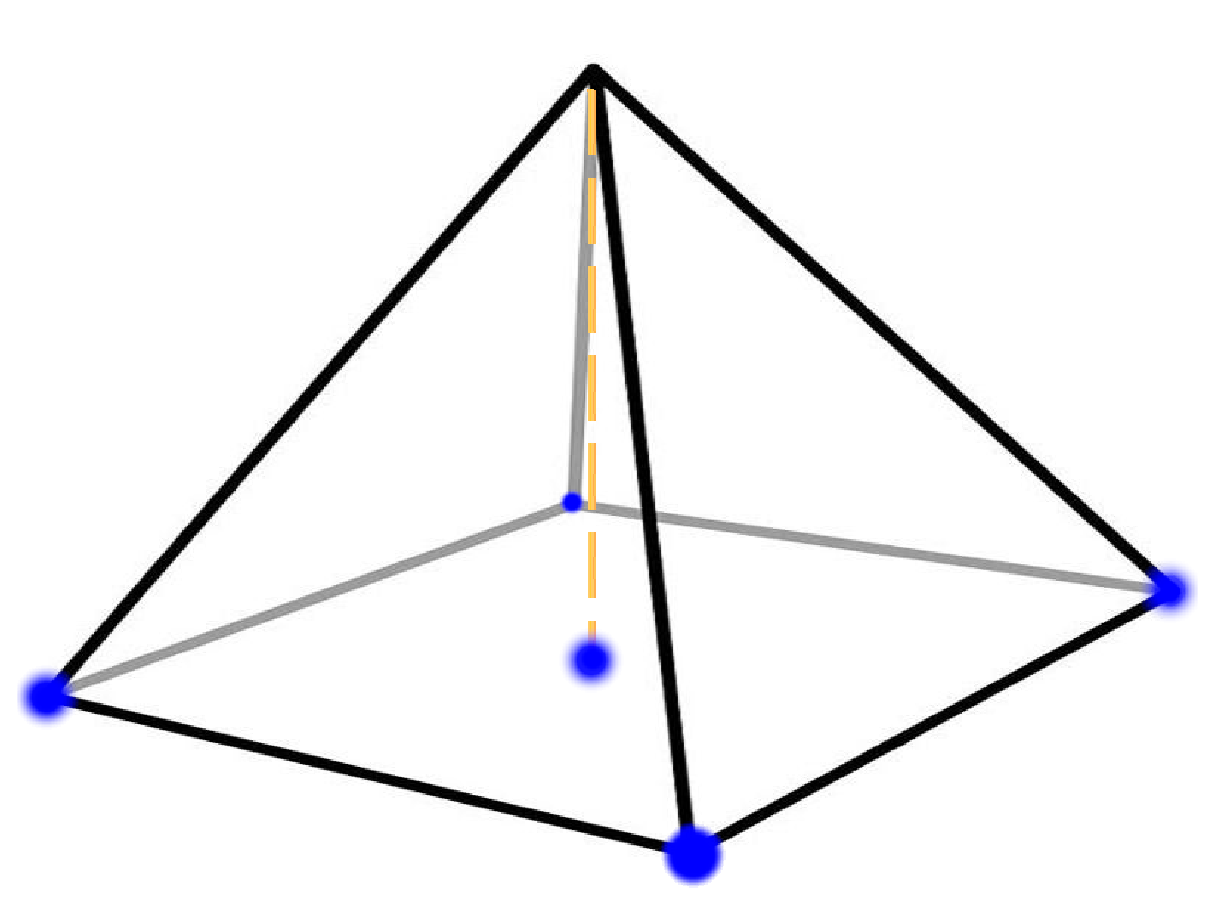
\includegraphics[width=0.5\linewidth]{figuras/piramide.eps}\\
  \caption{
Función de forma piramidal utilizada para producir las variaciones 
en el coeficiente de absorción. Esta función vale uno en el punto $\x_{\ell_1,\ell_2}$ 
y se anula a partir de los primeros vecinos de la grilla discreta.}
 \label{fig:priamid}
\end{figure}
 La función piramidal discretizada es aproximada como un producto 
 de deltas de Kronecker $\delta a_{\ell_1,\ell_2}=\delta_{r,\ell_1}\times\delta_{s,\ell_2}$.
 Llamando $\nabla_a g(\x_{\ell_1,\ell_2})$ al valor del gradiente funcional 
 en la dirección $\delta a_{\ell_1,\ell_2}$, la versión discreta 
 de la ecuación~\eqref{gradient_fin} resulta
\begin{equation}
\nabla_a g(\x_{\ell_1,\ell_2})  \sim -\sum_{m,j}  \lambda_{\ell_1,\ell_2,m,j}u_{\ell_1,\ell_2,m,j} \Delta \theta \Delta x \Delta y \Delta t,
\label{eq:FDwin22}
\end{equation}
donde $\lambda_{\ell_1,\ell_2,m,j}\sim
\lambda(\x_{\ell_1,\ell_2},\theta_m,t_j)$ y 
$u_{\ell_1,\ell_2,m,j} \sim u(\x_{\ell_1,\ell_2},\theta_m,t_j)$. 
Cabe notar que la ecuación~\eqref{eq:FDwin22} representa 
la derivada funcional para una única dirección $\delta a_{\ell_1,\ell_2}$ 
correspondiente a la componente $(\ell_1,\ell_2)$ del gradiente funcional discreto, 
donde el gradiente total discretizado estará dado por las perturbaciones en todas las direcciones posibles
\begin{equation}
\nabla_a g(\x)  = \left( \nabla_a g(\x_{1,1}), \nabla_a g(\x_{1,2}), \ldots, \nabla_a g(\x_{N_x+1,N_y+1})   \right).
\label{eq:grad_total}
\end{equation}
En el método adjunto, la evaluación de la ecuación~\eqref{eq:FDwin22} 
para todas las componentes $(\ell_1,\ell_2)$ del gradiente funcional requiere 
únicamente la resolución de un problema directo de transporte, y de 
su correspondiente problema adjunto para cada función generalizada $q=q_i$. 
En cambio, el uso de la ecuación~\eqref{eq:ObjFD} demanda la resolución de 
un número mucho más grande de problemas directos, donde debe evaluarse 
la resolución de $(N_x+1)\times (N_y+1)$ problemas de transporte, uno 
para cada perturbación del coeficiente $a(\x)$ en el dominio discretizado. 
Cabe mencionar también que el método adjunto requiere el almacenamiento 
en memoria de las soluciones completas a los problemas directos y adjunto de transporte 
para varios pasos temporales para realizar las integrales correspondientes~\eqref{eq:FDwin22}. 
El algoritmo paralelo propuesto en esta tesis es apropiado para este problema, ya que permite 
dividir simultáneamente el costo computacional y los requerimientos de memoria 
en sistemas distribuidos.
 
Como ilustración, en la figura~\ref{fig:gradient} se muestra 
el gradiente completo $\nabla_a g(\x_{\ell_1,\ell_2})$ para 
$1\leq \ell_1\leq N_x+1$ y $1\leq \ell_2\leq N_y+1$ 
para ciertos valores $\tilde G_{j,i}$, con una única fuente y 
un único detector ubicados en $\x_s=(1.5,0)$ y $\x_d=(1.0,0)$, 
respectivamente.

\begin{figure}[h!]
\centering
  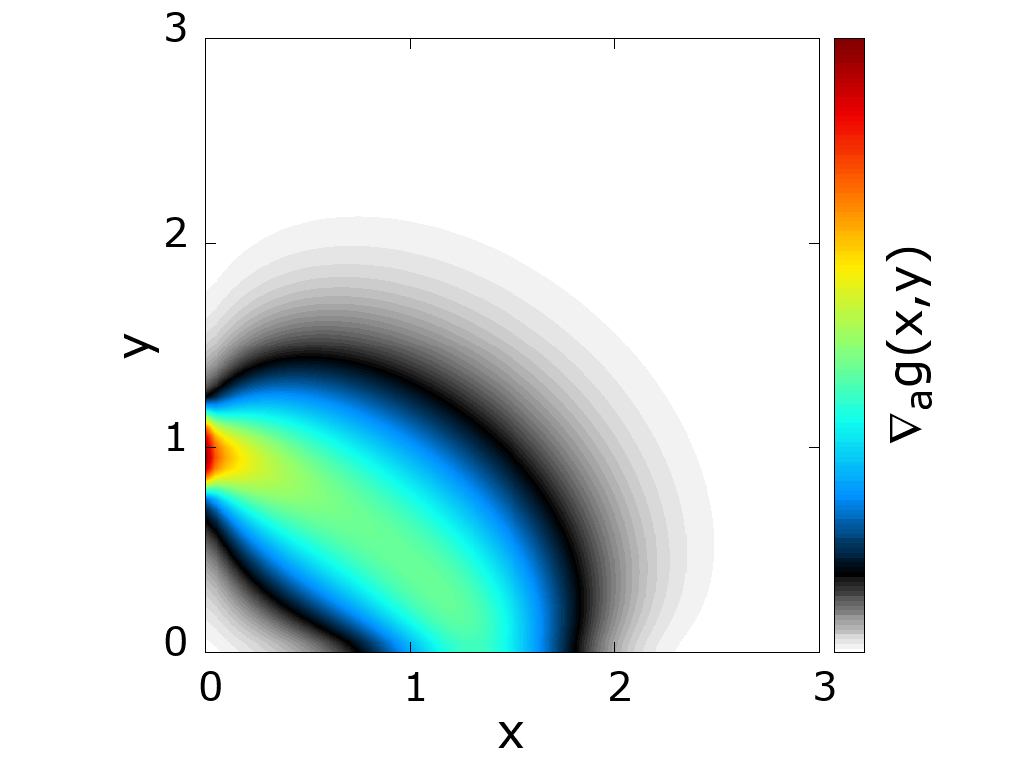
\includegraphics[width=0.5\linewidth]{figuras/gradient.png}
  \caption{
  Gradiente espacial~\eqref{eq:FDwin22} para todas 
  las direcciones discretas posibles $1\leq \ell_1\leq N_x+1$ y $1\leq \ell_2\leq N_y+1$, 
  con una única fuente y un único detector ubicados en $\x_s=(1.5,0)$ 
  y $\x_d=(0,1.0)$ respectivamente. Dado que se utilizaron 
  datos artificiales, la escala carece de sentido en esta figura, 
  y por eso no se muestra.}
 \label{fig:gradient}
\end{figure} 
 
\section{Datos sintéticos con fuentes láser pulsadas} 
\label{sec:sintetic} 

En las situaciones realistas en tomografía óptica, típicamente 
radiación colimada proveniente de una fuente láser incide en 
la superficie del dominio en estudio. En esta sección damos 
algunos detalles para el modelo directo utilizado  
en las siguientes secciones para la resolución del problema inverso. 
Modelamos la radiación colimada de las fuentes láser por medio 
de una función picuda de la variable $\theta$, donde el pico 
de esta función coincide con la dirección del láser incidente. 
Resolvemos la ecuación~ \eqref{eq:RTE} con condiciones de Fresnel, 
utilizando los parámetros $a(\x)=0.1$/cm, $b(\x)=20$/cm, $g=0.8$, 
$n_{\Omega}=1.4$ y $n_s=1.0$, en un dominio espacial $\Omega=[x_{\text{min}},x_{\text{max}}]\times[y_{\text{min}},y_{\text{max}}]=[0,3]\times[0,3]$. 

Mostraremos resultados para el método MB, y el método FMS. 
En el método MB empleamos una única fuente generalizada~\eqref{eq:RTEsources}, 
con $N_q=N_s=1$, centrada en $\x_{1,1}=(1.5,0)$, apuntando en la dirección 
normal a la superficie, de forma qué $\theta_{1,1}=\pi/2$, con $\sigma_{\theta}=\pi/4$. 
En esta configuración, una fuente láser inyecta radiación $y_{\text{min}}$ en la dirección 
normal a $\partial \Omega$ (Fig.~\ref{fig:photonflux}).
\begin{figure*}[h!]
\centering
  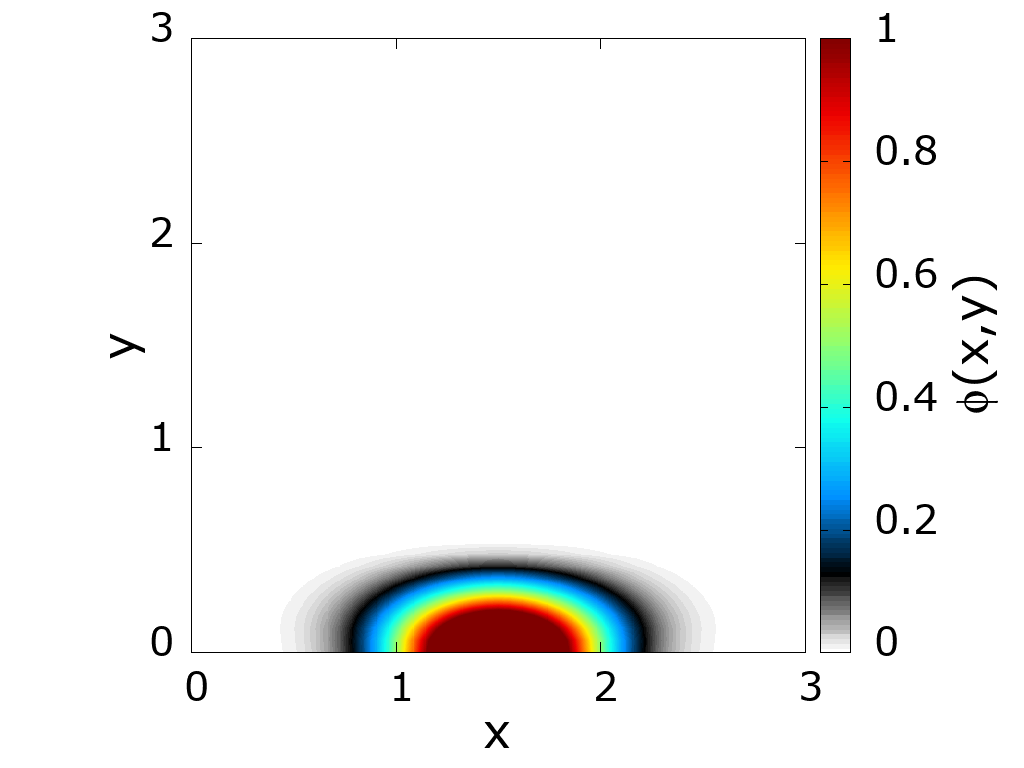
\includegraphics[width=0.325\textwidth]{figuras/sim_MB_t30.png}
  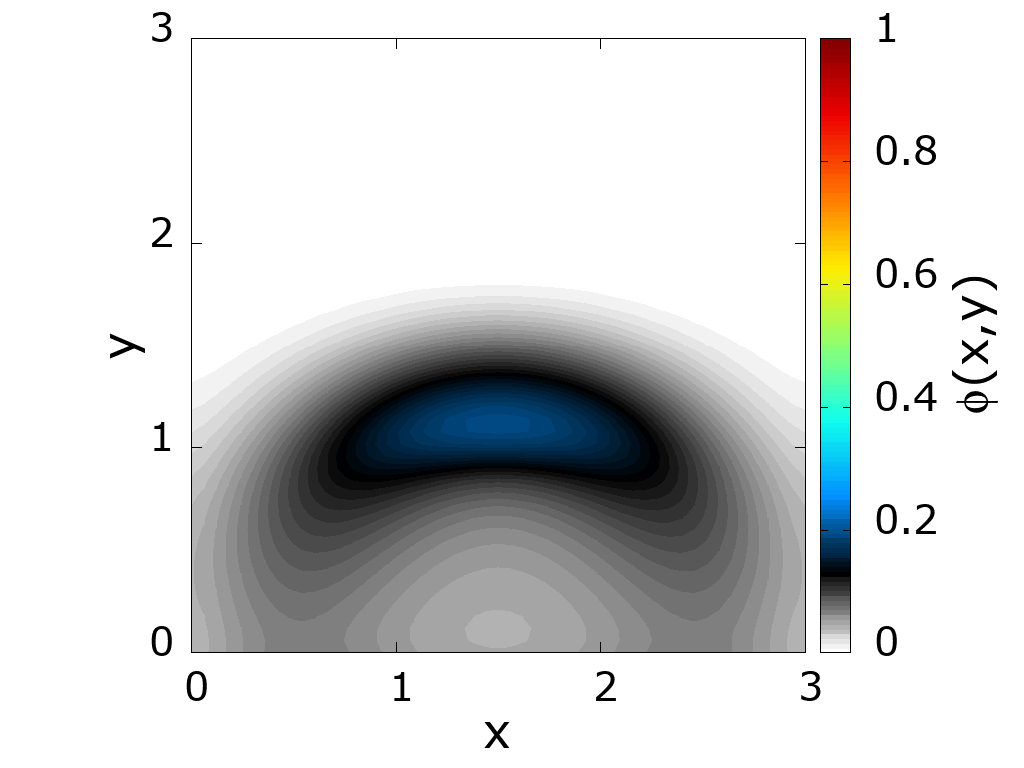
\includegraphics[width=0.325\textwidth]{figuras/sim_MB_t100.png}
  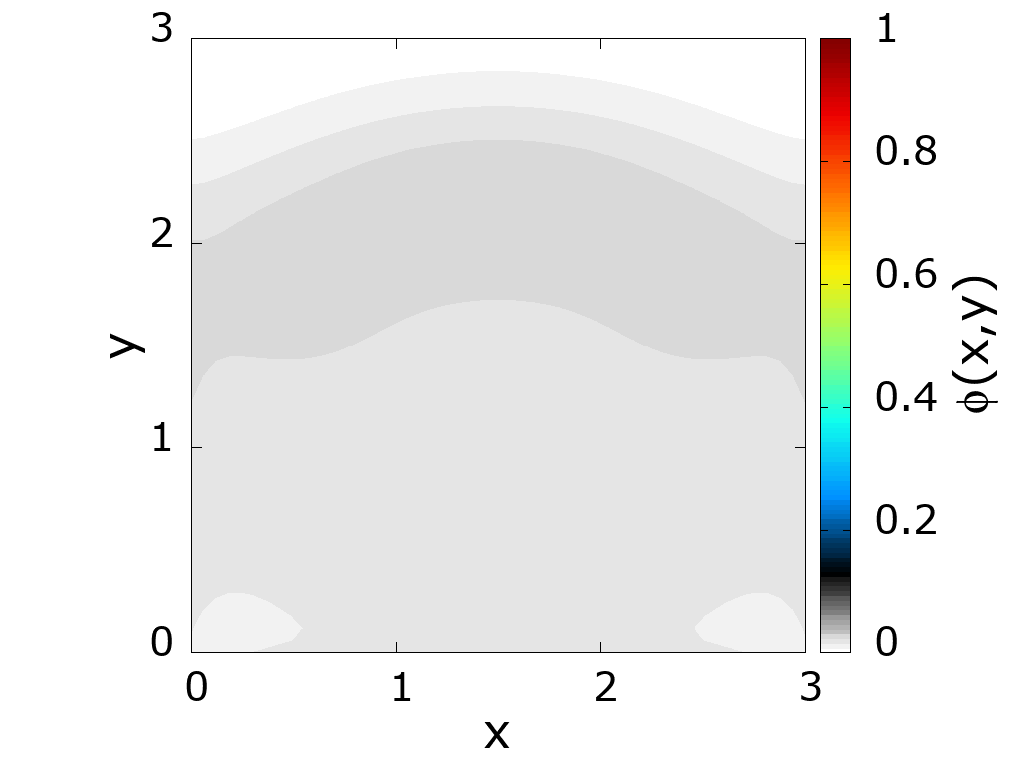
\includegraphics[width=0.325\textwidth]{figuras/sim_MB_t170.png}
  \caption{Simulación para el modelo directo MB utilizando 
  el método FC--DOM en paralelo~\ref{algfc} presentado en 
  la sección~\ref{subsec:FC-DOM}. En la figura se muestra el 
  flujo escalar $\phi(\x,t)$, ec.~\eqref{eq:photondensity} para tres tiempos 
  diferentes utilizando el método MB con una única fuente generalizada. De 
  izquierda a derecha se tiene $t=30$ps, 
$t=100$ps y $t=170$ps, para una fuente láser 
inyectando radiación en  $\x_s=(1.5,0)$cm. La figura muestra la evolución 
temporal de una ``onda de flujo de fotones'' difusos.}
 \label{fig:photonflux}
\end{figure*}
 
Para el método FMS, utilizamos una única fuente generalizada, con cuatro 
fuentes superpuestas, de forma qué $N_q=1$ y $N_s=4$. Cada fuente inyecta 
radiación en la dirección normal a $\partial \Omega$ a través del 
centro de las caras, con retardos temporales $\tau=200$ps entre fuentes sucesivas, 
comenzando con la fuente ubicada en $y_{\text{min}}$, seguida de la fuente 
en $y_{\text{max}}$, luego la ubicada en $x_{\text{min}}$ y finalmente 
se enciende la fuente en $y_{\text{max}}$ (Fig.~\ref{fig:photonflux2}).   
 

\begin{figure*}[h!]
\centering
  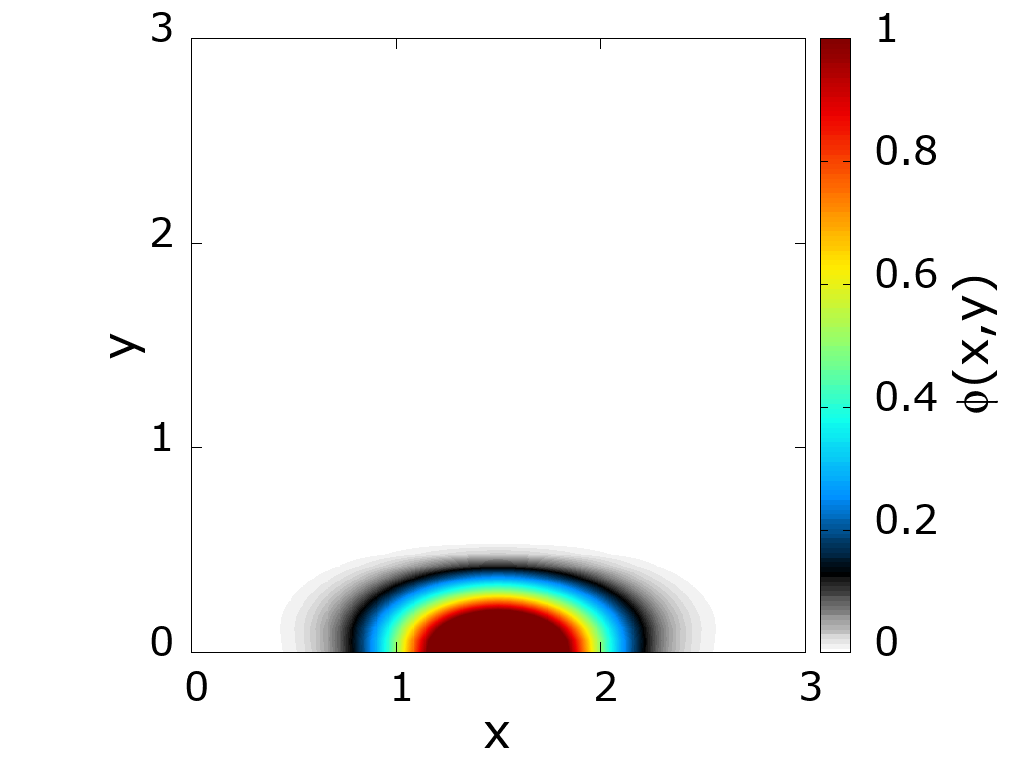
\includegraphics[width=0.325\textwidth]{figuras/sim_FMS_t30.png}
  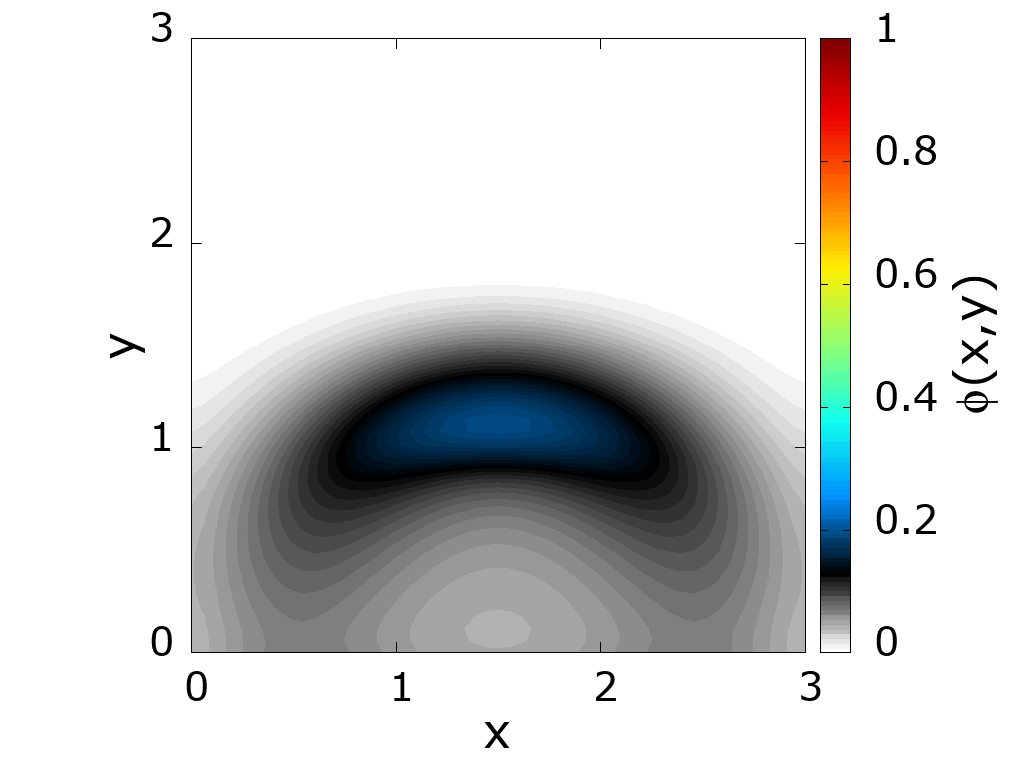
\includegraphics[width=0.325\textwidth]{figuras/sim_FMS_t100.png}
  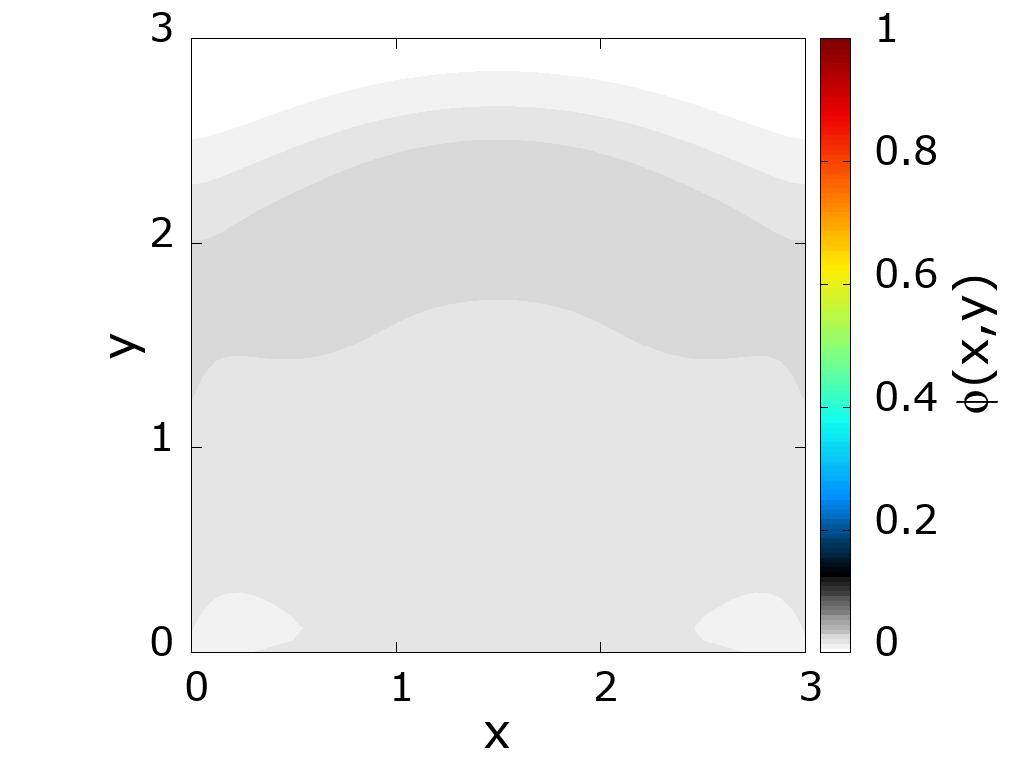
\includegraphics[width=0.325\textwidth]{figuras/sim_FMS_t170.png}\\
  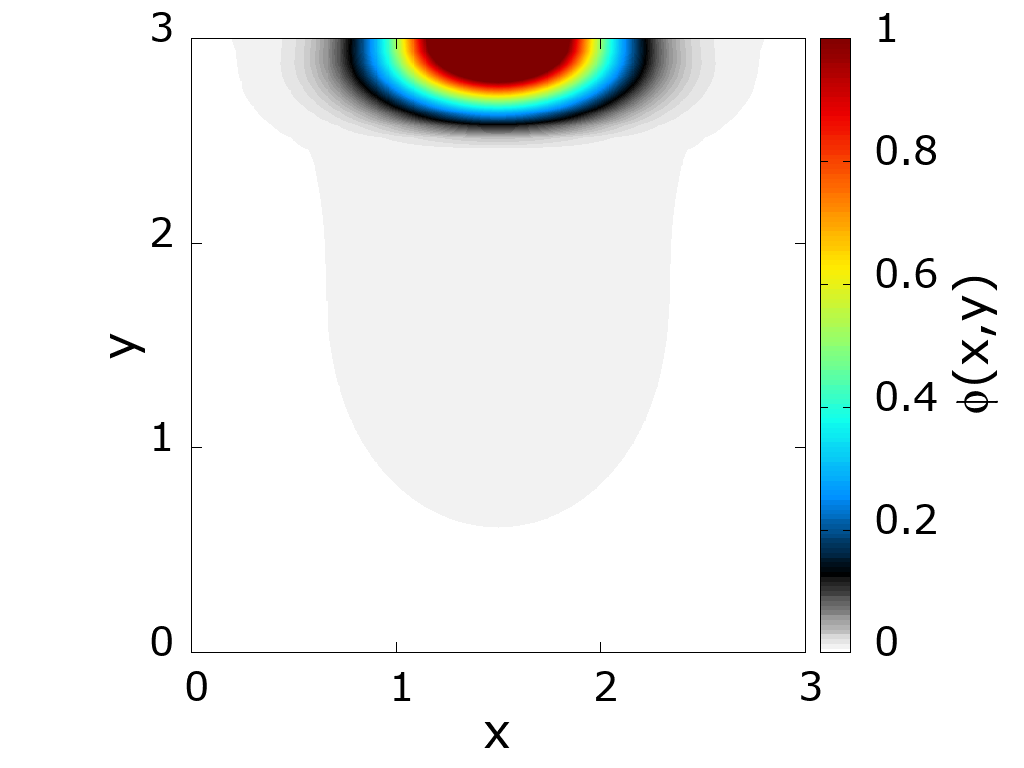
\includegraphics[width=0.325\textwidth]{figuras/sim_FMS_t230.png}
  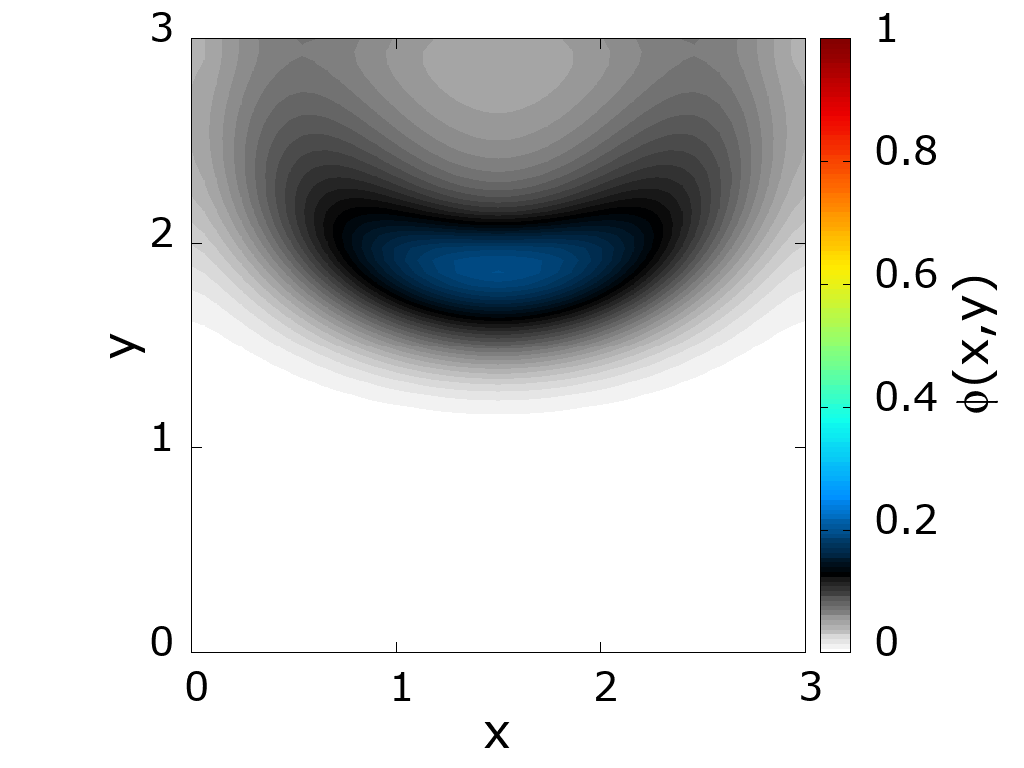
\includegraphics[width=0.325\textwidth]{figuras/sim_FMS_t300.png}
  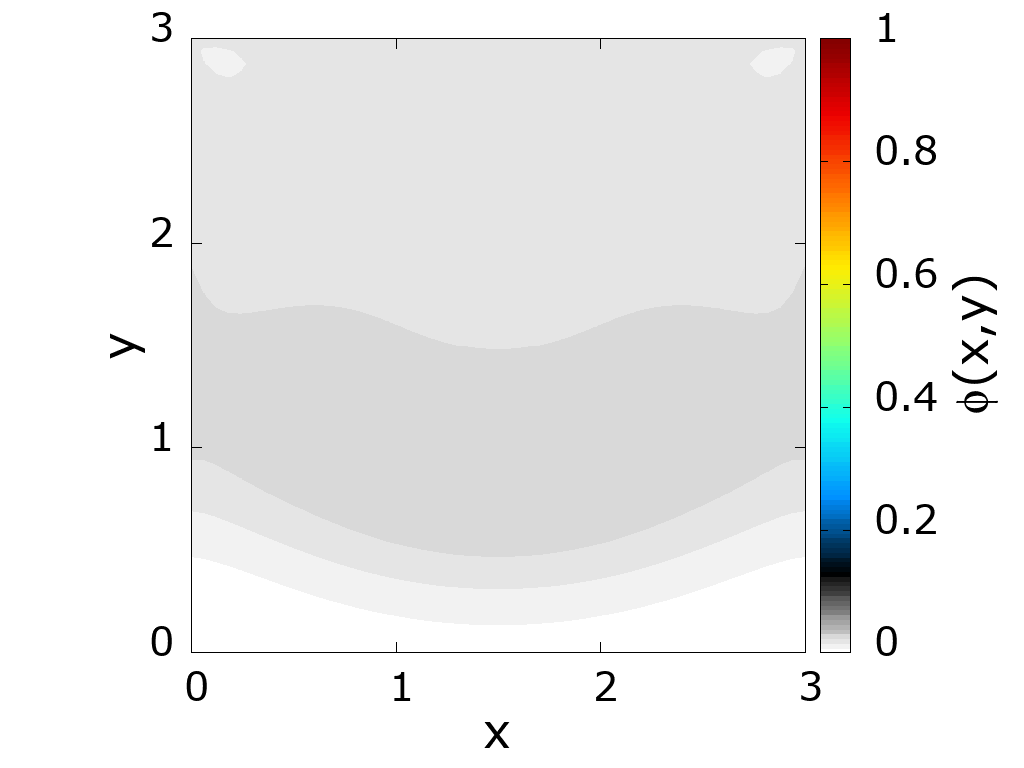
\includegraphics[width=0.325\textwidth]{figuras/sim_FMS_t370.png}\\
  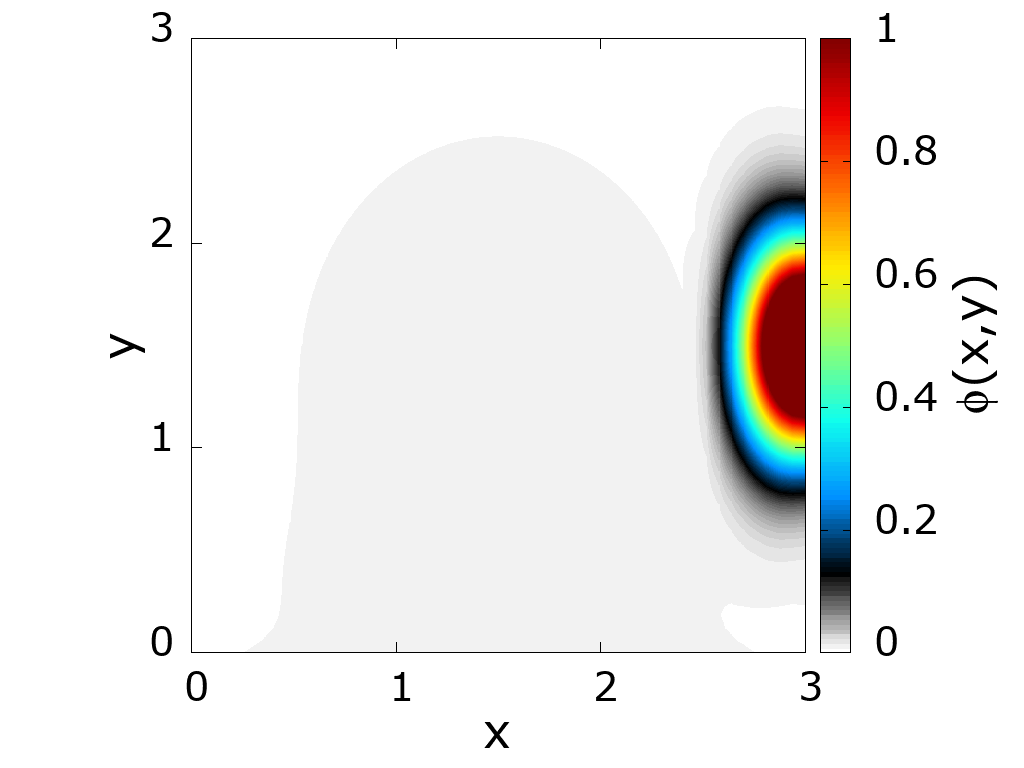
\includegraphics[width=0.325\textwidth]{figuras/sim_FMS_t430.png}
  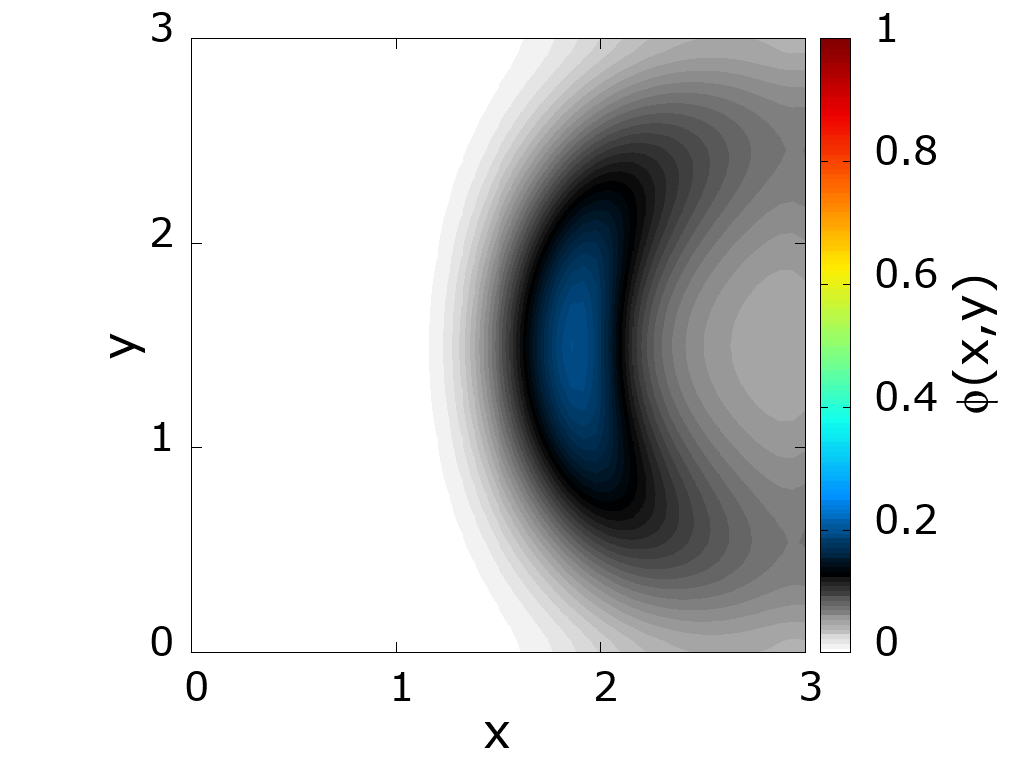
\includegraphics[width=0.325\textwidth]{figuras/sim_FMS_t500.png}
  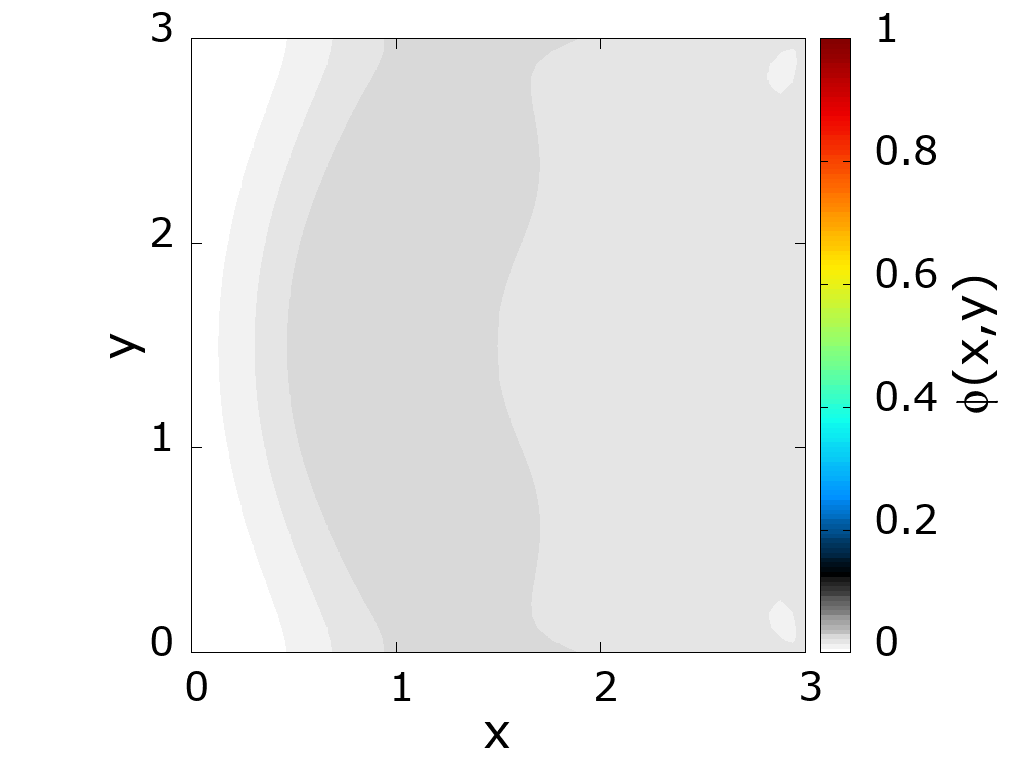
\includegraphics[width=0.325\textwidth]{figuras/sim_FMS_t570.png}\\
  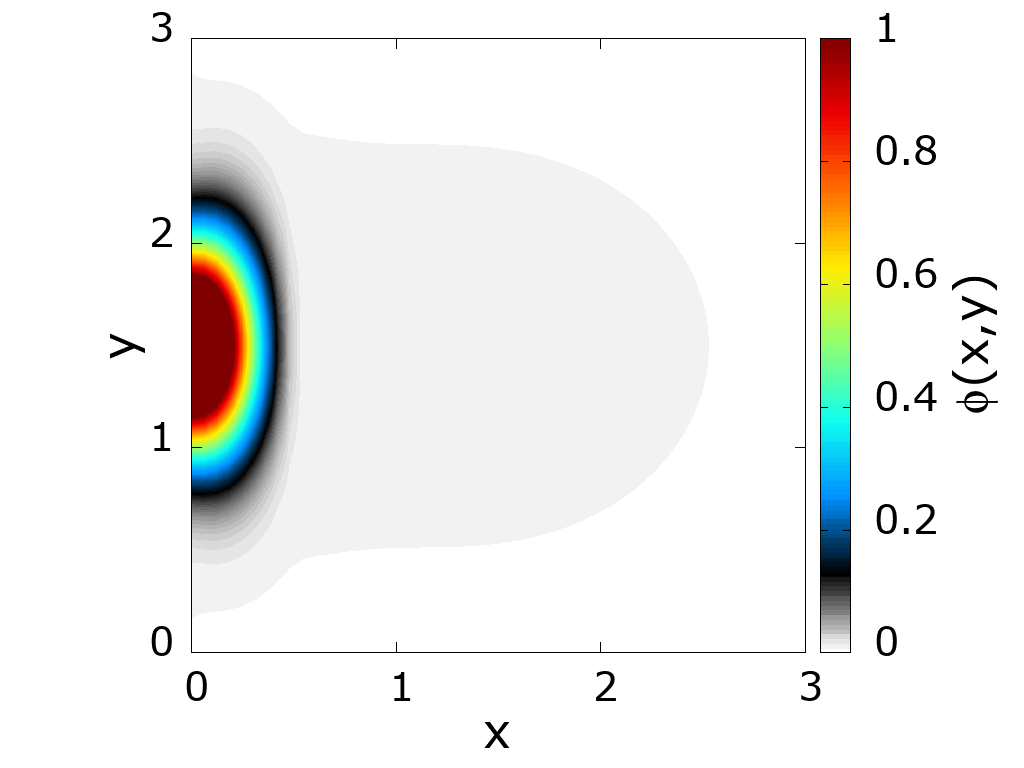
\includegraphics[width=0.325\textwidth]{figuras/sim_FMS_t630.png}
  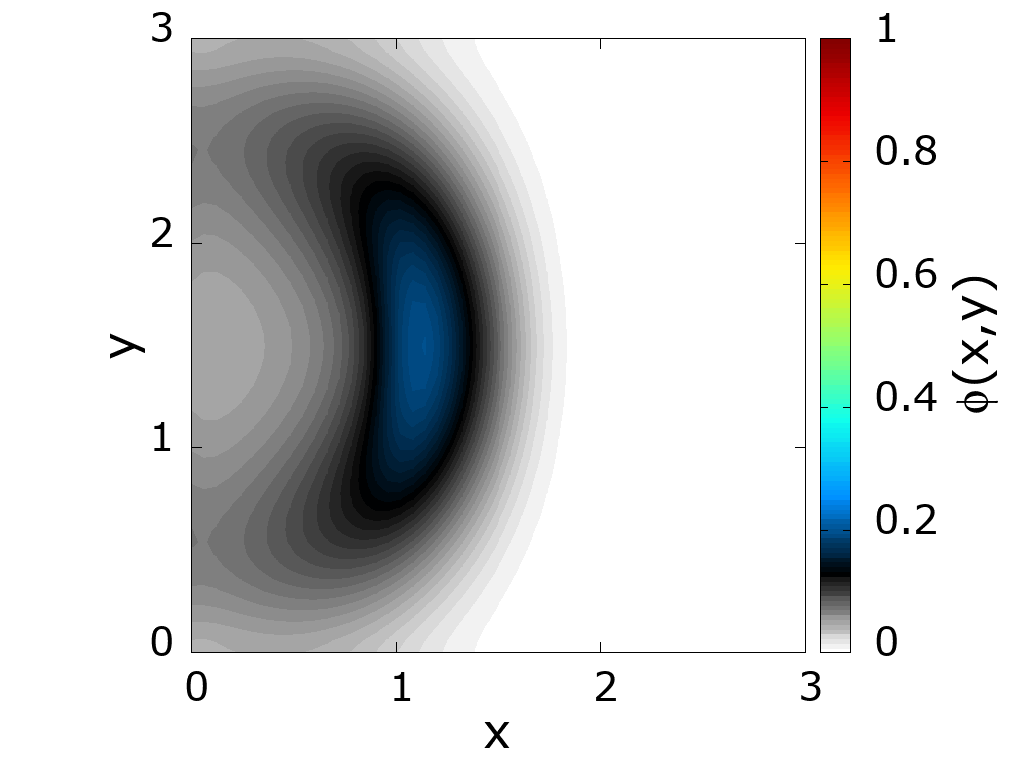
\includegraphics[width=0.325\textwidth]{figuras/sim_FMS_t700.png}
  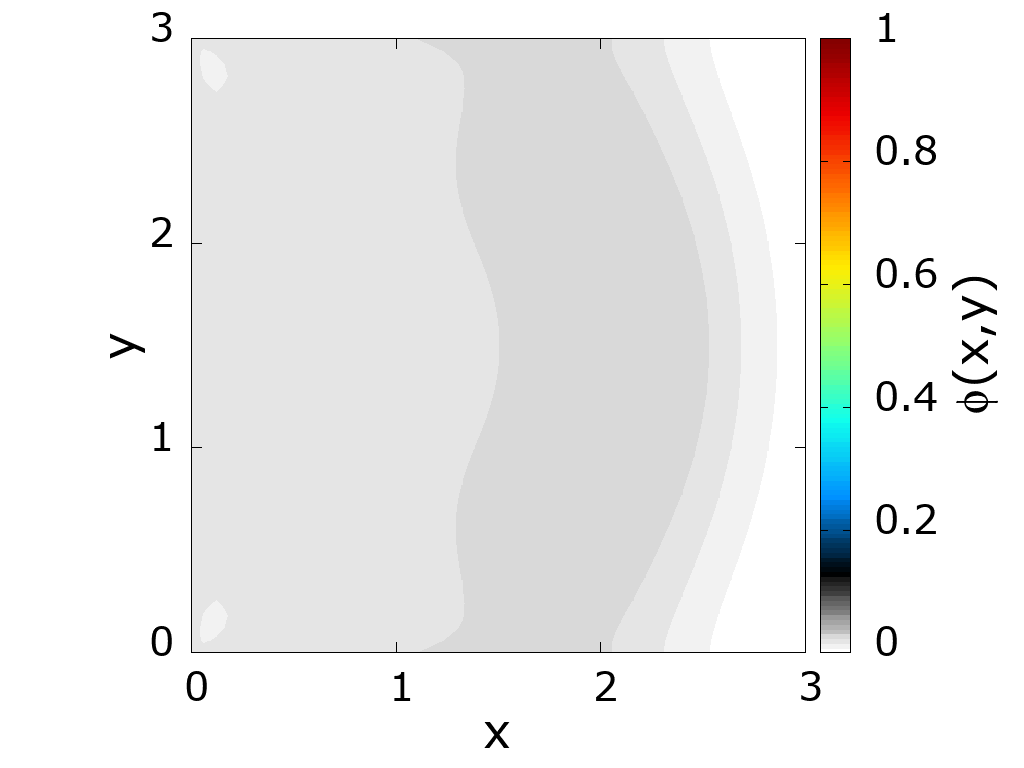
\includegraphics[width=0.325\textwidth]{figuras/sim_FMS_t770.png}
  \caption{Simulación para el modelo directo FMS utilizando 
  el método FC--DOM en paralelo~\ref{algfc} presentado en 
  la sección~\ref{subsec:FC-DOM}. En la figura se muestra el 
  flujo escalar $\phi(\x,t)=\phi(\x)$, ec.~\eqref{eq:photondensity} para tiempos 
  diferentes utilizando el método FMS con una única fuente generalizada 
  que contiene cuatro fuentes láser superpuestas, con tiempos de retraso $\tau=200$ps. De 
  izquierda a derecha y de arriba hacía abajo, se tiene $t=30$ps, $t=100$ps y $t=170$ps, 
   $t=230$ps, $t=300$ps y $t=370$ps,  $t=430$ps, $t=500$ps y $t=570$ps, 
    $t=630$ps, $t=700$ps y $t=770$ps.}
 \label{fig:photonflux2}
\end{figure*}

Para las reconstrucciones numéricas presentadas en la sección siguiente, utilizamos 
datos ``sintéticos'', esto es, datos generados de manera numérica 
con el algoritmo FC--DOM, para un dado 
coeficiente $a(\x)$. Dado que en situaciones realistas se espera 
que los datos experimentales presenten ruido, agregamos a los 
datos sintéticos un 10\% de ruido aleatorio a los datos sintéticos simulados 
utilizados en las reconstrucciones del problema inverso. 


Como puede observarse en la figura~\ref{fig:photonflux2}, para el método 
MB, dado que cada fuente láser individual es tratada mediante una simulación 
independiente de las otras fuentes, cada señal originada por los fotones 
transportados en el medio participante desde el láser hasta los detectores 
se encuentra desacoplada de la señal de las otras fuentes. En el método 
FMS, en cambio, las señales de todas las fuentes láser individuales 
aparece mezclada en los detectores.  El rol de los retardos temporales 
utilizados en el método FMS es desacopla en algún grado para 
un dado detector las señales 
originadas por fuentes láser individuales proveniente desde diferentes lugares.  

\begin{figure}[h!]
\centering
  \includegraphics[width=0.48\linewidth]{figuras/detread_sweep.eps}
  \includegraphics[width=0.48\linewidth]{figuras/detread_prop.eps}
  \caption{Lectura del detector $G[u_1]$ en la ec.~\eqref{eq:OpMed} para 
  una única fuente generalizada del método MB, y una fuente generalizada con 
  $N_s=4$ para el métofo FMS, antes y después de agregar un 10\% de ruido aleatorio 
  a la señal. El detector utilizado se ubicó en  $\x_d=(3.0,2.25)$. Cada fuente 
  láser individual se ubicó en el centro de las caras del dominio cuadrado. 
  Como puede observarse, en el método FMS las lecturas de los detectores 
  aparecen mezcladas. Utilizamos un retraso temporal  $\tau=200$ps entre las fuentes 
  ubicadas en las diferentes caras.}
 \label{fig:detread}
\end{figure}

\section{Algoritmo para la resolución del problema inverso}
\label{sec:inversesolv}

Como se indico anteriormente, el algoritmo propuesto en esta tesis para la resolución del 
problema inverso incorpora, en particular, la estrategia FMS, basada 
en el uso de fuentes que se aplican en un único problema directo, 
en lugar de la estrategia MB utilizada previamente en la literatura. 
En el método MB, por cada fuente láser deben realizarse un par 
de simulaciones para el problema directo y el problema adjunto, 
para luego combinar los resultados para obtener el gradiente utilizado 
en el método lm-BFGS. En cambio, en el método FMS propuesto, 
se construye la función objetivo utilizado una única fuente 
generalizada que contiene a todas las fuentes láser, de forma tal 
que se utiliza un único par de simulaciones para los problemas directos 
y adjuntos, lo cual, como se demuestra en la sección~\ref{sec:inverseres} 
(de manera cualitativa en las figuras~\ref{fig:itdet} y~\ref{fig:ithead} 
y de forma cuantitativa en las figuras~\ref{fig:reconst} y~\ref{fig:rechead}) 
reduce los tiempos de computo para el problema inverso de manera significativa 
(\eg en un factor de seis en la figura~\ref{fig:ithead}), sin que se 
produzca un deterioro en la calidad de la imagen obtenida. 

Buscamos el coeficiente de absorción que minimiza la ec.~\eqref{eq:FObjpr}  
sujeto a las restricciones $a^l(\x) \leq a(\x) \leq a^u(\x) \forall \x$, \ie, buscamos 
el coeficiente $a(\x)$ que es solución del problema 
\begin{equation}
\begin{split}
\begin{aligned}
a(\x)=\text{argmin}_{a^l \leq \widetilde a(\x) \leq a^u} \Lambda[a]
\end{aligned}
\end{split}
\label{eq:minprob}
\end{equation}

Las restricciones impuestas en el proceso de minimización están dadas 
por propiedades generales conocidas del coeficiente de absorción ($a^l(\x)\ge 0$ 
es una condición física que siempre debe cumplirse), y por cierto conocimiento 
del coeficiente, obtenido previamente por otras técnicas tomográficas, lo 
cual reduce el espacio de soluciones admisibles al problema de minimización~\eqref{eq:minprob}.

El algoritmo para la resolución del problema inverso~\ref{algfcinv},
procede de la siguiente manera. A partir de una estimación inicial $a^0(\x)$ para el
coeficiente de absorción y utilizando las lecturas de los detectores experimentales
$\widetilde{G}_{j,i}$, con $j=1, \ldots,N_d$ y $i=1,\ldots,N_q$, se resuelven
los problemas directos y adjuntos~\eqref{eq:RTE}
y~\eqref{eq:AdjointProblem}, a partir de lo cual se calcula el gradiente 
funcional~\eqref{eq:FDwin22}. El gradiente funcional 
se pasa al algoritmo lm-BFGS, que devuelve una actualización para 
coeficiente de absorción $a^1(\x)$ que reduce las diferencias entre
las lecturas de los detectores experimentales y los valores para los detectores simulados.
La iteración de este procedimiento converge, mediante el método lm-BFGS, al mínimo 
de la función objetivo~\eqref{eq:FObjpr}.

El algoritmo para la solución del problema inverso de transporte radiativo, 
para un dado número de iteraciones $i_{\text{max}}$, se presenta en forma de pseudocódigo en el 
algoritmo~\ref{algfcinv}. En este algoritmo, $C \in \mathbb{R}$ representa un criterio 
de convergencia preestablecido. El algoritmo se itera mientras el valor 
de la función objetivo esté por encima de dicho criterio de convergencia.
\begin{algorithm}
\caption{Algoritmo para la resolución del problema inverso en paralelo}
\label{algfcinv}
\begin{algorithmic}[1]
\State Dar una estimación inicial $a^0(\x)$
\State \textbf{para} $i=1,\ldots,i_{\text{max}}$ \textbf{hacer}
\State \hskip0.5em \textbf{para} cada fuente generalizada $q_j, j = 1,\ldots,N_q$ \textbf{hacer}
\State \hskip0.75em Resolver el problema directo por medio del algoritmo~\ref{algfc}
\State \hskip0.75em Evaluar ec.~\eqref{eq:FObjpr}, sí $ \Lambda[a] < C $ ir a \ref{al:end}.
\State \hskip0.75em Resolver el problema adjunto mediante el algoritmo~\ref{algfc}
\State \hskip0.5em\textbf{terminar}
\State \hskip0.5em Construir el gradiente ec.~\eqref{eq:FDwin22}
\State \hskip0.5em Llamar al algoritmo lm-BFGS para actualizar el coeficiente $a^{i+1}(\x)$.       
\State \label{al:end} \textbf{terminar} con $a(\x)=a^i(\x)$
\end{algorithmic}
\end{algorithm}


\section{Reconstrucciones numéricas}
\label{sec:inverseres}
En esta sección aplicamos los algoritmos desarrollados 
en las secciones previas al problema inverso en tomografía óptica. 
Los problemas inversos en tomografía óptica que consideramos 
conciernen a configuraciones en las cuales se buscan inclusiones 
sobre un tejido de ``fondo'' que se asume conocido. Esta situación describe, 
\eg, los excesos en la absorción de la radiación originados 
por la presencia de hemoglobina oxigenada en el cerebro, 
producida por la respuesta hemodinámica debido a la activación 
de una región determinada del cerebro~\cite{Boas2001,bluestone2001,Arridge1999,Hernandez2020}, 
para aplicaciones en neurociencias, 
o el exceso de hemoglobina oxigenada originada por la presencia de un tumor 
para aplicaciones en diagnósticos médicos~\cite{Althobaiti2017,Guven2003,Zhu2005,Zhu2010,Fujii2016b}.

La primera demostración que haremos ilustrará una aplicación potencial 
de la técnica de tomografía óptica para el diagnóstico 
de un paciente para el cual se dispone de una imágen por resonancia magnética (MRI)
del cuello (fig.~\ref{fig:mriim}). Describimos una situación teniendo 
en mente la aplicación potencial para el estudio de la evolución de la metástasis 
en una región específica del cuerpo (el cuello), tiempo después 
de haber adquirido la imagen MRI. Similarmente, el procedimiento 
podría utilizarse para seguir la evolución del tratamiento de un tumor en esta región. 
La portabilidad y el bajo costo de los sistema de tomografía óptica 
hace que estos dispositivos sean mucho mas accesibles para el diagnóstico 
que las imágenes obtenidas por sistemas MRI, para monitorear 
la evolución del tratamiento y el avance de un tumor de forma regular. 

En las referencias~\cite{Fujii2016b,Fujii2016} se realizó un estudio sobre el problema directo de la propagación de la luz en el cuello humano. Aquí presentamos un modelo similar,
 y extendemos la idea para el estudio 
de la convergencia del problema inverso siguiendo las lineas de las referencias~\cite{Fujii2016b,Fujii2016} con la intención de capturar 
algunas de las características mas importantes del cuello humano, 
manteniendo una geometría simple. 

Estudiaremos la convergencia por iteración del algoritmo~\ref{algfcinv} 
para un número variable de fuentes y detectores, para una dada configuración. 
Para evaluar la convergencia en el proceso de reconstrucción cuantificamos 
el error en la norma $L^2$ definido como
\begin{equation}
\begin{split}
\begin{aligned}
E(i)=\sqrt{\frac{\int_{\Omega}(a^v(\x)-a^i(\x))^2  d\x}{\int_{\Omega}a^v(\x) d\x}}
\end{aligned}
\end{split}
\label{eq:errl2}
\end{equation}
donde $E(i)$ corresponde al error en la norma $L^2$ para la iteración $i$, 
donde $a^v(\x)$ es el coeficiente de absorción ``verdadero'', y $a^i(\x)$ 
es el coeficiente de absorción obtenido por el algoritmo~\ref{algfcinv} 
en la iteración $i$-ésima. 

Buscaremos la existencia de un tumor en el tejido blando. 
Los coeficientes de la columna vertebral, la médula espinal, y la tráquea 
se mantendrán fijos en el proceso de reconstrucción, con $a^l(\x)=a^u(\x)=a(\x)$ 
en estas regiones, con los coeficientes dados para cada tipo de tejido correspondiente, 
los cuales se presentan en la tabla~\ref{tab:cuello}, y fueron tomados de las referencias~\cite{Bashkatov2011,Dehaes2011,Fujii2016}.

\begin{table}[h!]
\caption{Propiedades ópticas para el modelo de cuello humano}
\vspace{-0.3cm}
\begin{center}
\begin{tabular}{ccccccc}
\hline
Órgano & ~ $a[1/cm]$ & ~ & $b[1/cm]$ ~ & $g$ ~ & $n_{\Omega}$ \\
\hline
Tejido blando & ~$0.3$ & ~ & $80$ ~ &$0.9$ ~  & $1.4$ \\
Tráquea & ~$0.0$ & ~ & $0.0$ ~ &$0.0$ ~ &  $1.0$\\
Columna vertebral & ~$0.25$ & ~ & $148$ ~ &$0.9$   ~ &  $1.4$ \\
Médula espinal & ~$0.17$ & ~ & $882$ ~ &$0.9$  ~ &  $1.4$ \\
\hline
\end{tabular}
\label{tab:cuello}
\end{center}
\end{table}
Para simplificar el modelo, tomamos el coeficiente de refracción 
de la traquea cómo $n_{\Omega}=1.4$. Esto evita las dificultades 
encontradas para el modelado de la interfase entre la traquea y el tejido blando, 
el cual para un modelado mas preciso requiere tener en cuenta la reflexión 
de Fresnel en esta interfase geométricamente compleja. Otras simplificaciones 
adicionales utilizadas consistieron en no considerar los vasos sanguíneos, y en la 
simplificación de la geometría del cuello, el cual se tomo como una geometría 
cuadrada.

Por otra parte, fijamos el valor  $a(\x)=a^l(\x)=a^u(\x)$ 
al valor del fondo en las proximidades de los bordes, para puntos 
a una distancia menor a $0.5$cm. Este procedimiento genera una mejor 
convergencia en el problema de reconstrucción del coeficiente $a(\x)$, y previene 
la amplificación de los errores numéricos, originados por la existencia 
de las capa límite~\cite{Gaggioli2021} discutidas en la sección~\ref{sec:blayer}. 
La resolución de la capa límite en el problema multidimensional exige de métodos 
numéricos más sofisticados que escapan al alcance de esta tesis. 

Aplicamos el algoritmo para la reconstrucción del coeficiente 
de absorción, y comparamos los métodos MB y FMS propuesto en este trabajo. 
Para ello, producimos datos sintéticos de la forma descripta en la sección~
\ref{sec:sintetic}, donde agregamos un 10\% de ruido aleatorio a los datos obtenidos 
para los detectores mediante las simulaciones numéricas, de forma de obtener 
resultados que se acerquen a una situación experimental real.

Como mencionamos anteriormente, la situación que simulamos es una en la cual se buscan inclusiones sobre 
cierto ``fondo'' conocido. La situación que ilustramos en este primer caso corresponde 
a los excesos de absorción 
originados por la presencia de hemoglobina oxigenada debido a la presencia de un tumor 
en el tejido, lo cual encuentra aplicaciones tanto en el diagnostico de la enfermedad, así 
como en el seguimiento del tratamiento de la misma.

El mínimo $a^l$ para el coeficiente de absorción vendrá dado 
por los valores del ``fondo'' del tejido analisado (que se asume conocido \textit{a priori}). 
El límite superior estará dado por valores típicos del coeficiente de absorción 
para el tejido que se está examinando, y lo fijaremos en $a^u=1$.

La imagen MRI es tomada como el coeficiente inicial $a^0(\x)$
para la iniciación de las iteraciones. 

\begin{figure}[h!]
\centering
  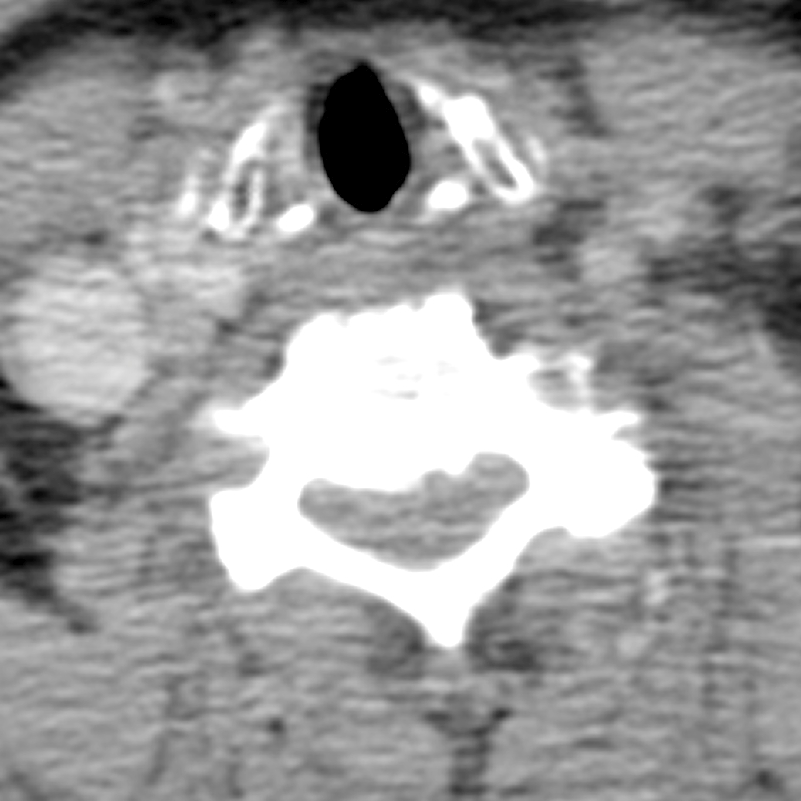
\includegraphics[width=0.25\linewidth]{figuras/neck_mri.png} 
  \caption{Imagen de Resonancia Magnética~\cite{CCommons} para el modelo de cuello humano empleado. } 
 \label{fig:mriim}
\end{figure}

\begin{figure}[h!]
\centering
  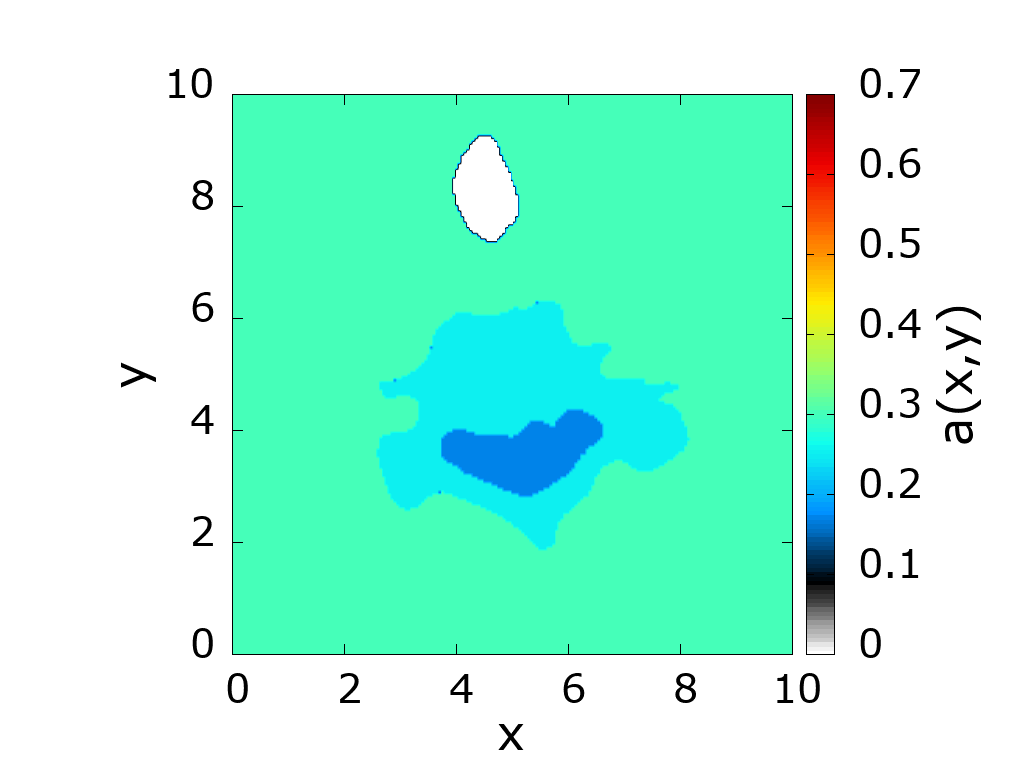
\includegraphics[width=0.48\linewidth]{figuras/neck_i.png} 
  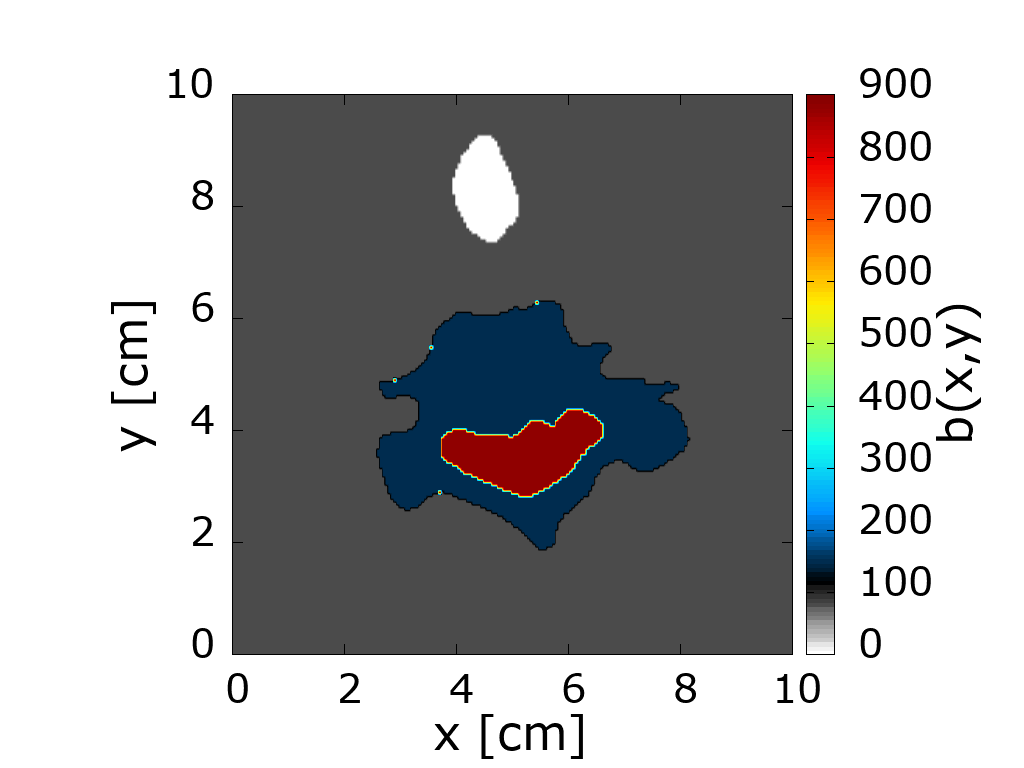
\includegraphics[width=0.48\linewidth]{figuras/neckmss_scatt.png} 
  \caption{Izquierda: coeficiente de absorción 
  generado a partir de la imagen~\ref{fig:mriim}, el cual fue utilizado como el coeficiente 
  inicial $a^0(\x)$ en las reconstrucciones del coeficiente de absorción para éste modelo. 
  Derecha: coeficiente de dispersión para el modelo de cuello humano.
  Los coeficientes de absorción y dispersión 
  para los distintos órganos fueron tomados de las referencias\cite{Bashkatov2011,Dehaes2011,Fujii2016}. } 
 \label{fig:mriimc}
\end{figure}

En esta demostración, para el método FMS empleamos una única fuente generalizada 
la cual contiene multiples fuentes láser. Las diferentes fuentes láser 
contenidas en esta única fuente generalizada iluminan el borde del dominio $\partial \Omega$ 
en la dirección normal al mismo, inyectando la radiación que atraviesa 
el medio participante, sensándolo, y luego es recolectada por los detectores. 
La configuración que elegimos para la activación de las fuentes es tal 
que se activan de manera simultánea una fuente por cara. 
Utilizamos un retraso temporal de $300$ps para fuentes vecinas ubicadas 
en una misma cara. En detalle, para el caso con 16 fuentes, fijamos 
$\tau_{1,1}=0$ps para las fuentes simultáneas ubicadas en $\x_1^1=(2.0,0.0)$, 
$\x_1^2=(10.0,2.0)$, $\x_1^3=(8.0,10.0)$,  $\x_1^4=(0.0,8.0)$, donde utilizamos 
el supraíndice para indicar las diferentes fuentes láser individuales, y el subíndice 
para indicar el teimpo de retraso temporal correspondiente $\tau_{k,1}$ (ver la ecuación~\eqref{eq:RTEsources}).
El resto de las fuentes se configuran de la siguiente manera: 
$\x_2^1=(4.0,0.0)$, 
$\x_2^2=(10.0,4.0)$, $\x_2^3=(6.0,10.0)$,  $\x_2^4=(0.0,6.0)$ con $\tau_{2,1}=300$ps, 
$\x_3^1=(6.0,0.0)$, 
$\x_3^2=(10.0,6.0)$, $\x_3^3=(4.0,10.0)$,  $\x_3^4=(0.0,4.0)$ con $\tau_{3,1}=600$ps 
and $\x_4^1=(4.0,0.0)$, 
$\x_4^2=(10.0,4.0)$, $\x_4^3=(6.0,10.0)$,  $\x_4^4=(0.0,6.0)$ con retraso temporal $\tau_{4,1}=900$ps. 

Este arreglo fue guiado por la idea de utilizar en el métofo FMS como fuentes simultaneas 
aquellas que están geométricamente más alejadas unas de otras. Debido 
al decaimiento exponencial en la onda de densidad de fotones difusos (ver fig.~\ref{fig:photonflux}), es esperable que cada fuente láser tenga un efecto despreciable en las lecturas de los detectores cercanos a otras fuentes geométricamente lejanas, 
aún cuando fueron activadas de manera simultánea. Para dar tiempo suficiente 
a la relajación de las ondas de fotones producidas por las fuentes activadas 
de forma más tardía, cada simulación directa en el método FMS fue evolucionada 
hasta el tiempo final $t_{\text{max}}=1400$ps. Para los casos en los que se utilizaron 
un número menor de fuentes, la configuración para la activación de las mismas 
fue similar. Para el método MB, cada simulación directa fue evolucionada hasta el tiempo 
final $t_{\text{max}}=600$ps, con los detectores y las fuentes ubicados en las mismas 
posiciones que las utilizadas en el método FMS, y utilizando las mismas grillas numéricas, 
e igual número de procesadores en cada caso.

\begin{figure*}[h!]
\centering
  \includegraphics[width=0.49\textwidth]{figuras/detsSweep.eps}
  \includegraphics[width=0.49\textwidth]{figuras/detsMSS.eps}
\\
    \vspace{0.3cm}
  \includegraphics[width=0.49\textwidth]{figuras/sourcesSweep.eps}
  \includegraphics[width=0.49\textwidth]{figuras/sourcesMSS.eps}
  \caption{Convergencia obtenida para el error en la norma $L^2$ ec.~\eqref{eq:errl2} 
  del coeficiente de absorción con respecto al número de iteraciones, 
  para un número variable de detectores (arriba) y de fuentes láser (abajo), para los métodos 
  MB y FMS. 
   A la izquierda: 
  error en la norma $L^2$ ec.~\eqref{eq:errl2} para 100 iteraciones del método MB. 
  Derecha:error en la norma $L^2$ ec.~\eqref{eq:errl2} para 100 iteraciones del método FMS. 
  Para las simulaciones en el panel superior se utilizaron 16 fuentes láser. Para 
  las simulaciones en el panel inferior, se utilizaron 36 detectores.}
 \label{fig:itdet}
\end{figure*}


Como puede apreciarse en la figura~\ref{fig:itdet}, los métodos MB y FMS 
presentan propiedades de convergencia similares para un número variable 
de fuentes y detectores. Sin embargo, para el caso con 16 fuentes, 
el método FMS tomó  $12689$ segundos para llegar a las 100 iteraciones, 
del algoritmo~\ref{algfcinv}, mientras que el método MB tomó $88093$ segundos, 
dando una aceleración en la reconstrucción por un factor cercano a siete. 
En la figura además se aprecia que incrementar el número de fuentes y de detectores 
genera una mejora considerable en la convergencia del problema inverso 
para un número fijo de iteraciones. El número de fuentes tiene un impacto 
mayor en las reconstrucciones que el número de detectores. 
Esto puede entenderse de la siguiente manera, dado que la función de las fuentes 
es producir los fotones que viajan a través del medio participante para sensarlo 
y finalmente ser recolectados en los detectores, si bien los detectores son necesarios 
para conocer la distribución de los fotones en el medio, en el problema adjunto~\eqref{eq:AdjointProblem} 
son las diferencias $(G_j[u_i]-\widetilde{G}_{j,i})$ los que cumplen el rol de las fuentes, 
pero la intensidad de estas ``fuentes'' en el problema adjunto dependen de la cantidad 
de fotones originados en las fuentes láser que inyectan la radiación en el medio participante 
para llegar luego a los detectores. Puede argumentarse que por esta misma razón, 
es mas importante la cantidad de fuentes que inyectan radiación en el medio para sensar 
la totalidad de $\partial \Omega$, que si esas fuentes son simuladas en problemas 
directos separados, lo cual sugiere que el método FMS es una estrategia 
de optimización adecuada que permite ganar tiempo de cómputo aprovechando 
el uso de fuentes simultáneas en único problema directo.

\pagebreak
\begin{wrapfigure}{r}{0.48\textwidth}
%\begin{figure*}[h!]
\centering
  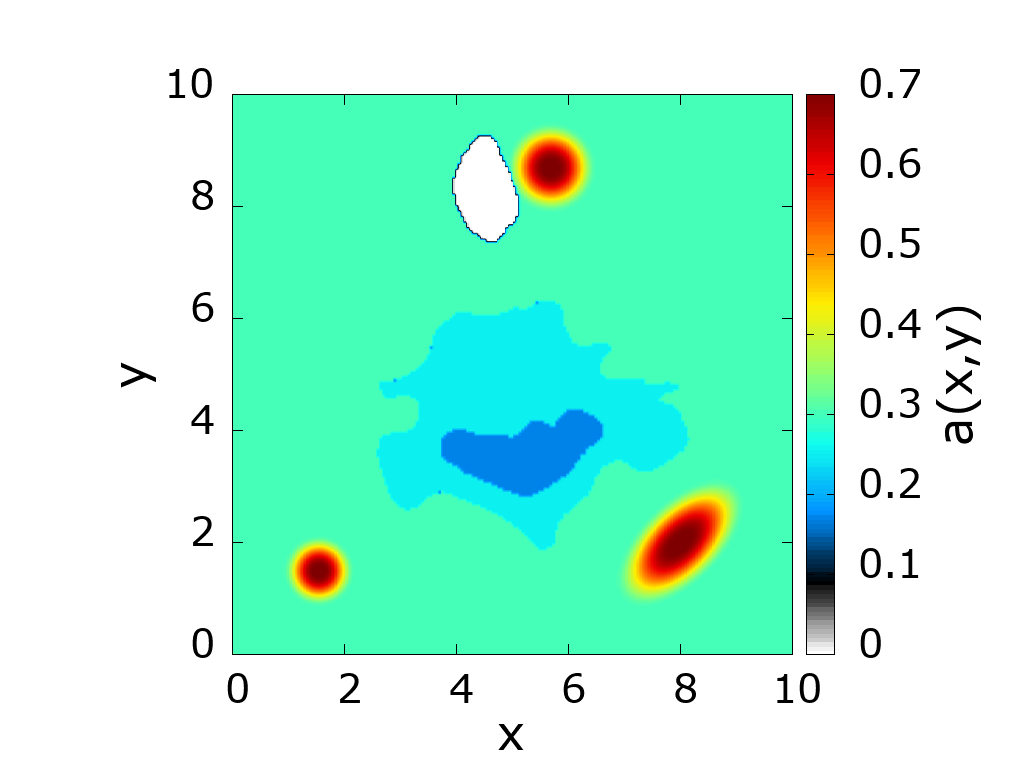
\includegraphics[width=0.45\textwidth]{figuras/necktrue.png}\\

  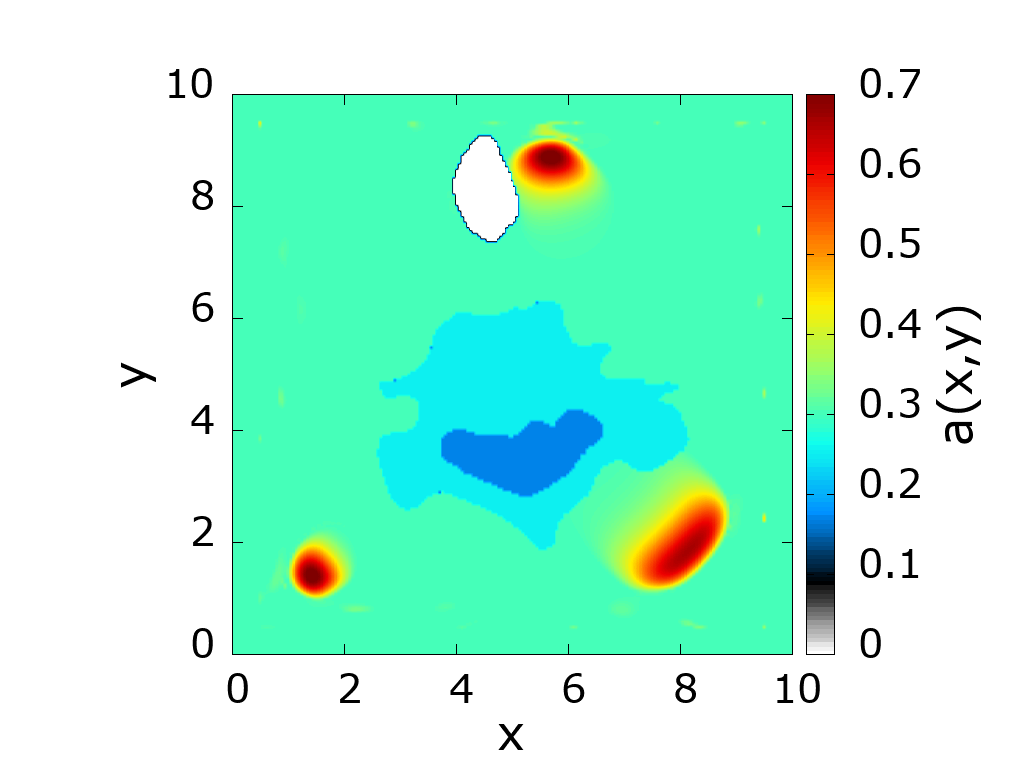
\includegraphics[width=0.45\textwidth]{figuras/necksweep.png}\\

  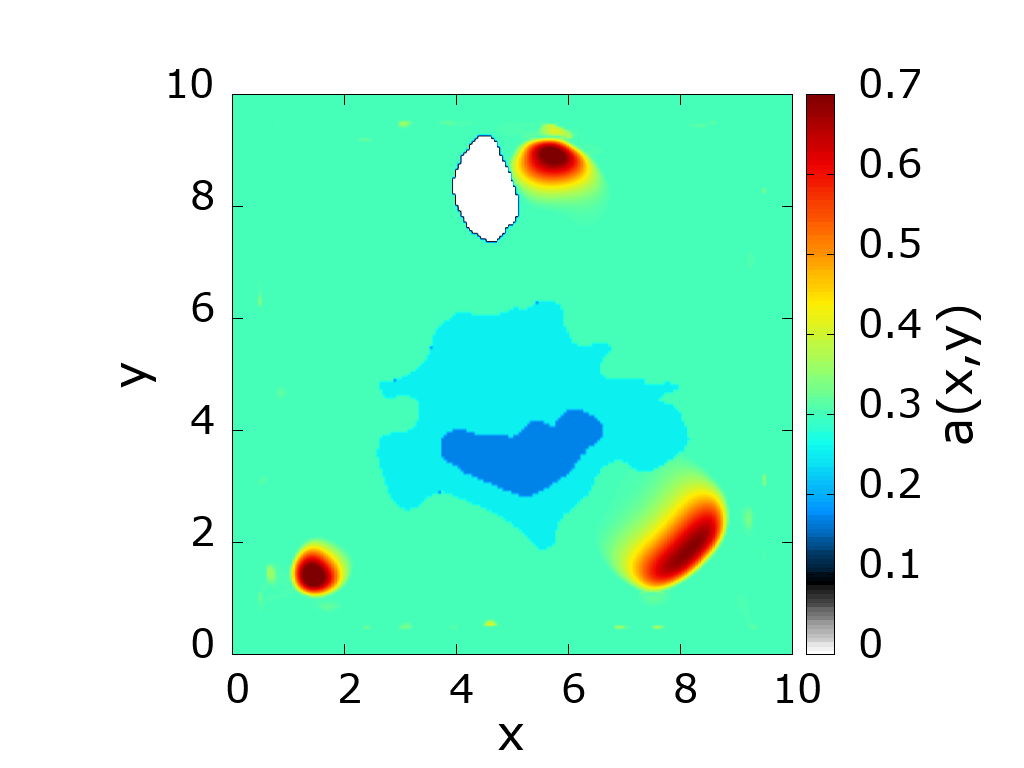
\includegraphics[width=0.45\textwidth]{figuras/neckmss.png}
  \caption{De arriba a abajo: coeficiente de absorción verdadero, y
  coeficientes de absorción obtenidos mediante resolución del problema inverso para 100 iteraciones de los métodos MB y FMS, respectivamente.}
 \label{fig:reconst}
%\end{figure*}
\end{wrapfigure}
En la figura~\ref{fig:reconst} mostramos el coeficiente de absorción verdadero, 
junto con los coeficientes de absorción obtenidos mediante la resolución del problema 
inverso empleando las estrategias MB y FMS, con 16 fuentes y 36 detectores 
para 100 iteraciones del algoritmo~\ref{algfcinv}. Como puede observarse, 
las reconstrucciones obtenidas por ambos métodos son de similares características. 

Finalmente, presentaremos una reconstrucción simulando un ``modelo de cabeza''. 
Para esta demostración, utilizaremos el modelo de cabeza similar 
a los utilizados en las referencias~\cite{Klose2002,Prieto2017}. 
Este modelo de cabeza simula la situación típica donde 
se utiliza tomografía óptica para estudiar la actividad hemodinámica 
en el cerebro humano, y captura la característica más importante 
en este contexto, el cual es la región ubicada entre el cráneo y el cerebro, 
la cual contiene un fluido de baja absorción y baja dispersión, conocido 
como fluido cerebroespinal. Esta región cumple la función de 
amortiguar al cerebro ane movimientos bruscos. Además, el fluido cerebroespinal 
se encarga de transportar nutrientes hacia el cerebro, y de
eliminar metabolitos.
Dado que el fluido cerebroespinal presenta coeficientes de absorción y de dispersión 
despreciables, la ecuación de difusión de fotones no es físicamente preciso para modelar 
el transporte de fotones en esta región, por lo cual debe emplearse la ecuación de transporte.
En la referencia~\cite{Prieto2017} se utilizan 16 fuentes, 4 por cara, para 
un modelo de cabeza similar. 
%\pagebreak
%\clearpage

\begin{figure}[h!]
\centering
  \includegraphics[width=0.5\linewidth]{figuras/l2err.eps}\\
  \caption{Evolución del error en la norma $L^2$ por iteración ec.~\eqref{eq:errl2} para el coeficiente de absorción, obtenido para el modelo de cabeza humana para los métodos MB y FMS.}
 \label{fig:ithead}
\end{figure}

\noindent Aquí emplearemos 32 detectores, con 8 detectores por cara, 
e igual número de fuentes. 
Mostramos el coeficiente de absorción después de 50 iteraciones del método MB, 
e iteramos el método FMS hasta obtener un error de convergencia similar en la norma $L^2$~\eqref{eq:errl2}. En estas reconstrucciones, nuevamente buscamos inclusiones 
sobre un fondo conocido, el cual es utilizado como estimación inicial $a^0(\x)$. 
La región del fluido cerebroespinal, así como la región por fuera del mismo, 
se asumen conocidos (dado que en estas regiones no puede ocurrir la activación cerebral), 
y se mantienen fijos durante el proceso de reconstrucción. Buscamos las inclusiones 
en la región circular interior, dado que es en esta región donde se encontraría 
el cerebro en una situación menos idealizada.

Para mostrar que también pueden emplearse otras estrategias de activación, 
en esta prueba utilizaremos una configuración diferente para la 
activación de las fuentes en el método FMS. Todas las fuentes ubicadas 
en una misma cara serán activadas de manera simultánea. En la notación 
utilizada anteriormente, tendremos $\x_1^1=(1.0,0.0)$, 
$\x_1^2=(2.0,0.0)$, $\x_1^3=(3.0,0.0)$, $\x_1^4=(4.0,0.0)$, con retardo temporal $\tau_{1,1}=0$ps. \looseness=-1
\begin{wrapfigure}{r}{0.48\textwidth}
\centering
  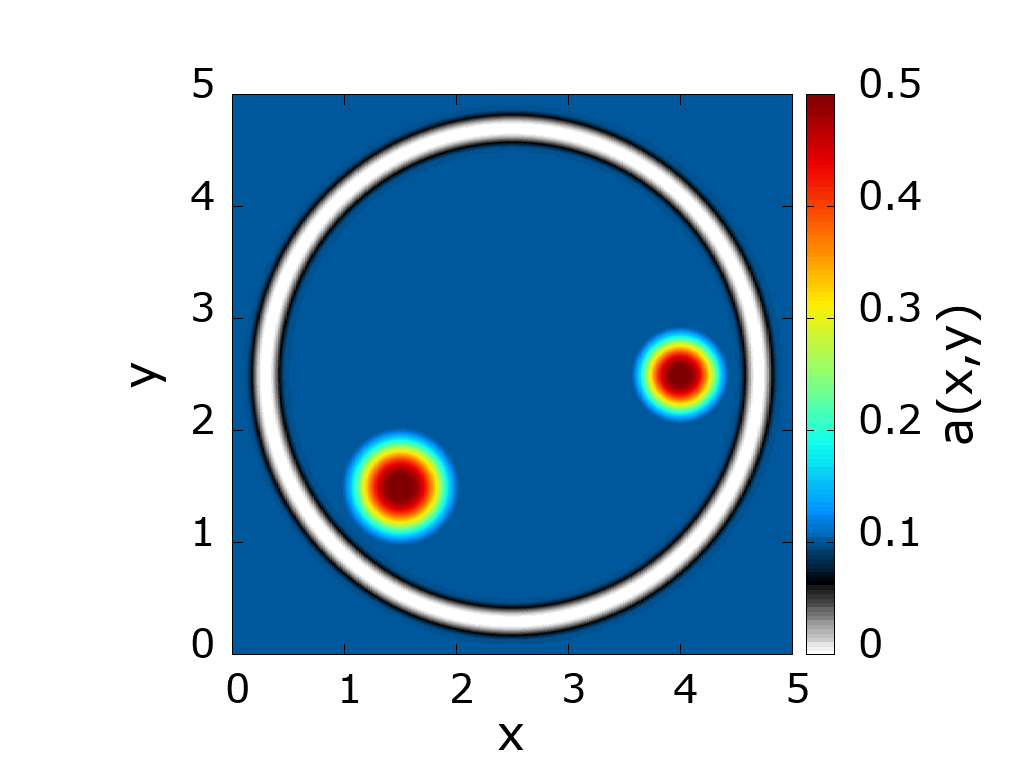
\includegraphics[width=0.45\textwidth]{figuras/head_true.png}\\
  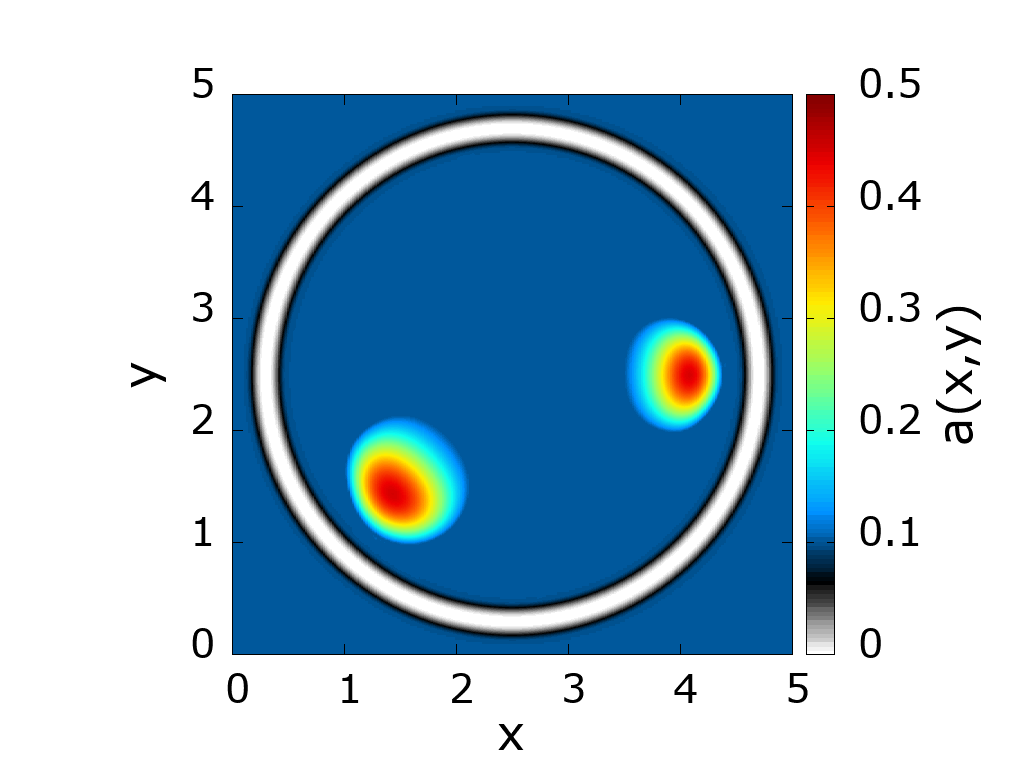
\includegraphics[width=0.45\textwidth]{figuras/head_sweep.png}\\
  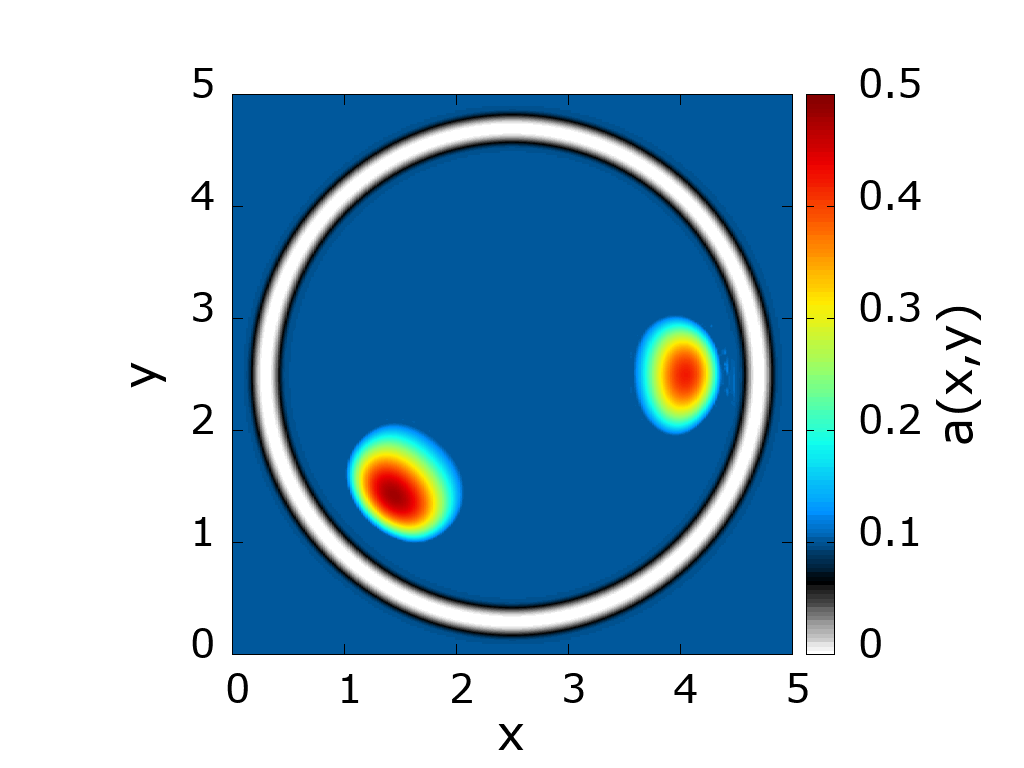
\includegraphics[width=0.45\textwidth]{figuras/head_ours.png}
  \caption{De arriba a abajo: coeficiente de absorción verdadero, y coeficientes de 
  absorción obtenidos para 50 iteraciones del método MB, y 79 iteraciones del métofo FMS.}
 \label{fig:rechead}
\end{wrapfigure}
Luego 
$\x_2^1=(1.0,5.0)$, 
$\x_2^2=(2.0,5.0)$, $\x_2^3=(3.0,5.0)$,  $\x_2^4=(4.0,5.0)$ con $\tau_{2,1}=100$ps, 
$\x_3^1=(5.0,1.0)$, 
$\x_3^2=(5.0,2.0)$, $\x_3^3=(5.0,3.0)$,  $\x_3^4=(5.0,4.0)$ con $\tau_{3,1}=400$ps 
y $\x_4^1=(0.0,1.0)$, 
$\x_4^2=(0.0,2.0)$, $\x_4^3=(0.0,3.0)$,  $\x_4^4=(0.0,4.0)$ con retardo temporal de $\tau_{4,1}=500$ps.
En la figura~\ref{fig:ithead} mostramos la evolución del error ec.~\eqref{eq:errl2} 
para los métodos MB y el método FMS propuesto. En la figura~\ref{fig:rechead} 
mostramos el coeficiente de absorción verdadero, y los obtenidos al final 
de la iteración para cada método.

En términos de tiempo computacional, las cincuenta iteraciones del método 
MB tomaron mas de seis veces que las setenta y nueve iteraciones del 
método FMS. Si los dos métodos fueran iterados igual número de iteraciones, 
se obtendrían reconstrucciones similares, con un detrimento en favor 
del método MB, pero con el método FMS realizando las iteraciones en casi un órden 
de magnitud más rápido. La calidad de las reconstrucciones han mostrado 
depender en la discretización numérica utilizada. En particular, 
si se utilizan menos direcciones discretas, se obtienen 
reconstrucciones de menor calidad para ambos métodos, 
posiblemente debido a la aparición del efecto de rayos 
en el interior de la región de baja absorción y dispersión. 

También es posible emplear otras estrategias de activación en el método 
FMS. A pesar de que no hemos explorado otras posibilidades, 
es posible incluir más fuentes generalizadas, con diferentes 
estrategias de activación cada una de ellas. 



